%------------------------------------------------------------------------------
% Template file for the submission of papers to IUCr journals in LaTeX2e
% using the iucr document class
% Copyright 1999-2013 International Union of Crystallography
% Version 1.6 (28 March 2013)
%------------------------------------------------------------------------------

%\documentclass[preprint]{iucr}              % DO NOT DELETE THIS LINE
\documentclass{iucr}              % DO NOT DELETE THIS LINE

\usepackage{siunitx}
\usepackage{color}
\usepackage{amsmath,amssymb}
\usepackage{mathtools}
\usepackage[normalem]{ulem}

% rotation table labels...
% see https://tex.stackexchange.com/questions/98388/how-to-make-table-with-rotated-table-headers-in-latex
\usepackage{adjustbox}
\usepackage{array}
\usepackage{booktabs}
\usepackage{multirow}

%
%




\newcommand{\todo}[1]{{\color{red}[TODO: "#1'']}}
\newcommand{\inblue}[1]{{\color{blue}#1}}
\newcommand{\inred}[1]{{\color{red}#1}}
\newcommand{\ingreen}[1]{{\color{green}#1}}
\newcommand{\soutred}[1]{{\color{red}\sout{#1}}}

\newcolumntype{R}[2]{%
    >{\adjustbox{angle=#1,lap=\width-(#2)}\bgroup}%
    l%
    <{\egroup}%
}
\newcommand*\rot{\multicolumn{1}{R{90}{1em}}
%
}% no optional argument here, please!


     %-------------------------------------------------------------------------
     % Information about journal to which submitted
     %-------------------------------------------------------------------------
     \journalcode{S}              % Indicate the journal to which submitted
                                  %   A - Acta Crystallographica Section A
                                  %   B - Acta Crystallographica Section B
                                  %   C - Acta Crystallographica Section C
                                  %   D - Acta Crystallographica Section D
                                  %   E - Acta Crystallographica Section E
                                  %   F - Acta Crystallographica Section F
                                  %   J - Journal of Applied Crystallography
                                  %   M - IUCrJ
                                  %   S - Journal of Synchrotron Radiation

\begin{document}                  % DO NOT DELETE THIS LINE

     %-------------------------------------------------------------------------
     % The introductory (header) part of the paper
     %-------------------------------------------------------------------------

     % The title of the paper. Use \shorttitle to indicate an abbreviated title
     % for use in running heads (you will need to uncomment it).

\title{Pairing transfocators under partially coherent x-ray beams}
%\shorttitle{Short Title}

     % Authors' names and addresses. Use \cauthor for the main (contact) author.
     % Use \author for all other authors. Use \aff for authors' affiliations.
     % Use lower-case letters in square brackets to link authors to their
     % affiliations; if there is only one affiliation address, remove the [a].

\cauthor[a]{Manuel}{Sanchez del Rio}{srio@esrf.eu}{address if different from \aff}
\author[a]{Rafael}{Celestre}
\author[a]{Juan}{Reyes-Herrera}
\author[a]{Philipp}{Brumund}
\author[a]{Marco}{Cammarata}

\aff[a]{European Synchrotron Radiation Facility, 71 Avenue des Martyrs, 38000 Grenoble \country{France}}
% \aff[b]{Second affiliation address}

     % Use \shortauthor to indicate an abbreviated author list for use in
     % running heads (you will need to uncomment it).

%\shortauthor{Soape, Author and Doe}

     % Use \vita if required to give biographical details (for authors of
     % invited review papers only). Uncomment it.

%\vita{Author's biography}

     % Keywords (required for Journal of Synchrotron Radiation only)
     % Use the \keyword macro for each word or phrase, e.g. 
     % \keyword{X-ray diffraction}\keyword{muscle}

%\keyword{infrared beamline}

     % PDB and NDB reference codes for structures referenced in the article and
     % deposited with the Protein Data Bank and Nucleic Acids Database (Acta
     % Crystallographica Section D). Repeat for each separate structure e.g
     % \PDBref[dethiobiotin synthetase]{1byi} \NDBref[d(G$_4$CGC$_4$)]{ad0002}

%\PDBref[optional name]{refcode}
%\NDBref[optional name]{refcode}

\maketitle                        % DO NOT DELETE THIS LINE

\begin{synopsis}
We simulate the focusing of partial coherent beams produced by fourth-generation storage rings using a new software tool, Wofry 1D, that implements coherent mode decomposition of undulator radiation in 1D. We observe changes in the focal spot of the focus when the numerical aperture is reduced by a slit. The pairing of two transfocators to assure a fixed focal position is studied and the resulting beam sizes analyzed. 
% In this paper we study the focal parameters (position, size, intensity) given by a partial coherent beam, where the NA and coherence fraction are controlled by an aperture. We analyze the focal position originated by a compound system of two lenses, CRLs or transfocators.
\end{synopsis}

\begin{abstract}
We simulate the focusing of partial coherent beams produced by fourth-generation storage rings. We used a new software tool to perform coherent mode decomposition of the undulator radiation in 1D. The analysis of a focusing system based on x-ray lenses, shows the shift and degradation of the focus when the numerical aperture is reduced by a slit. The pairing of two transfocators to assure a fixed focal position is studied in terms of beam sizes and coherent fraction. The results show that the synchrotron source imaged by two paired undulators is highly dependent on the aperture used to control the coherence fraction, and simple concepts based on geometrical optics cannot be applied. 
\end{abstract}


     %-------------------------------------------------------------------------
     % The main body of the paper
     %-------------------------------------------------------------------------
     % Now enter the text of the document in multiple \section's, \subsection's
     % and \subsubsection's as required.

\section{Introduction}
\label{sec:introduction}


Recent fourth-generation storage-ring-based X-ray synchrotron sources deliver photon beams with high brilliance and coherence. The transversal coherence of these beams is highly improved, in particular in the horizontal direction, with respect to previous 3$^{\text{rd}}$ generation sources. This has a beneficial impact for many applications requiring coherent beams, such as X-ray photon correlation spectroscopy, coherent diffraction imaging, propagation-based phase-contrast imaging, and ptychography (see, e.g. \cite{paganin_book}). On the other side, preserving wavefront quality requires better quality materials and optical surfaces in the active beamline components such as mirrors, gratings, crystals and lenses \cite{Yabashi, Roth2017}. Moreover, the interaction of the coherent beam with the optical elements produce diffraction that do affect their focusing power and resolving power of these elements. Let us consider, for example, the case of an ideally focusing system of focal length $f$ made by a mirror or lens that focuses the source into the image plane. The position of the focus with respect to the focusing element $q$ can be estimated by the lens equation $f^{-1}=p^{-1}+q^{-1}$, with $p$ the source-element distance. If the beam numerical aperture (NA) is reduced (for example by the finite dimension of the lens, mirror or by using a slit) the position and also the dimensions of the focal point changes due to diffraction. It has been shown \cite{Tanaka:85} that the focal position created by a Gaussian beam ``moves" towards the lens position when NA reduces. This shifting of the focal position is also relevant for synchrotron beamlines, as demonstrated by \citeasnoun{westfahl}. These authors noticed a shift of the horizontal focal position upstream from the position given by geometrical optics (see Fig. 7 in \citeasnoun{westfahl}) when the horizontal acceptance is reduced by a slit. Their numeric results from wavefront propagation using SRW \cite{codeSRW} including partial coherence agree with an analytical Gaussian Shell-model.

The diffraction effect at the slits and finite size of the optical elements not only shifts the focal point, but also changes the focal dimensions, as we will see later. These facts are critical when designing beamlines with several coupled focusing elements. We study this phenomenon applied to the project for the new ID18 beamline at the upgraded EBS-ESRF storage ring. This beamline will produce highly coherent beams of variable cross section at the sample position. Two refractive systems (transfocators) are paired to allow a varying focal size, whereas a slit placed upstream from the transfocators is used to control the coherent fraction. The optical matching of the transfocators is studied in detail, and it is strongly correlated with the slit aperture (or coherent fraction). To study the performances of such systems a new algorithm for coherent mode decomposition (CMD) of the undulator beams has been developed. This method is very fast allowing parametric simulations in a common laptop.

The high efficiency of the CMD software developed is obtained by implementing a 1D model, therefore studying separately the horizontal and vertical planes. The results of this model are verified against 2D models using Monte-Carlo multielectron propagation with SRW and also 2D coherent mode decomposition with COMSYL \cite{codeCOMSYL}. It is also found that ray-tracing simulations using the ``hybrid" method \cite{codeHYBRID} give good approximations to the correct results for these systems. 

The paper is organized as follows. Section~\ref{sec:theory} summarizes the methodology used for 1D coherent mode decomposition of undulator beams and their transport along the beamline. Section~\ref{sec:onelens} analyzes the focusing of partially coherent beams with a single refractive system (lens). Section~\ref{sec:twolenses} discusses the pairing of two refractive systems. Section~\ref{sec:complete-beamline} shows simulations for the full beamline and compares different methodologies for a selected case. We finish with a general discussion in Section~\ref{sec:discussion} and  concluding remarks in Section~\ref{sec:summary}. 


\section{One dimensional coherent mode decomposition of an undulator source and propagation along a beamline with lenses}\label{sec:theory}

For dealing with partially coherence beams produced by undulators in low-emittance storage rings we developed a 1D model of the CMD method that we previously developed in 2D \cite{glass2017}. The motivation for developing these new tools is to perform quick calculations (e.g., being able to perform parametric calculations in a laptop) with high accuracy in the simulation of the source and beam propagation. The separation of the real 2D wavefront in two separated 1D wavefronts is well justified for most synchrotron beamlines, where the cross-talk between these two directions is small. 
The tools developed here are included in the OASYS toolbox \cite{codeOASYS}, available as an WOFRY add-on. These tools can be used from the OASYS interface, which also creates scripts that can be later modified for performing parametric calculations and loops in batch runs. 


\subsection{Modeling the partial coherent emission of an undulator beam using coherent mode decomposition}

The electrons in a storage ring are statistically distributed, following in good approximation a Gaussian distribution in a 6-dimensional space (three spatial coordinates, two angles to define direction, and the electron energy). The radiation of the individual electrons will add incoherently for wavelengths smaller than the bunch lengths. This is the usual case for X-rays produced by storage ring-based sources, but not for free electron lasers. Therefore, each electron creates a wavefront (fully coherent) associated at a given photon energy. As a consequence, the overall radiation cannot be described deterministically. Statistical methods are then needed, like for describing the electron beam. This is the origin of partial coherence of the synchrotron emission. In an ideal storage ring of zero emittance, the electrons follow a filament beam so the emission by an insertion device (ID) would be fully coherent. When electron emittance is considered, the electrons contributing to the radiation have different initial conditions (in the 6-dimensional space) and the overall emission cannot be describe by a single wavefront, but by statistically distributed wavefronts, described by partial coherent optics.

The radiation is ``wide sense stationary" \cite{mandel_wolf} if it verifies some conditions, usually satisfied for light emitted by storage rings, but not for XFELs \cite{geloni2008}. These conditions can be summarized as
i) the electron bunch length being long enough (several times larger than the emitted wavelength),
ii) radiation is monochromatized 'not too much' (like by standard monochromators), and 
iii) the radiation frequency being large enough.
It is in this case all the coherent properties of the radiation can be described using $W$, the ``cross spectral density" (CSD), a complex function that measures the correlation of the electric field $E$ in two different spatial points at a given radiation frequency $\omega$. It can be mapped in a $(x,y)$ plane at a third coordinate $z$. At that plane, the CSD depends on 5 variables: 

\begin{equation}
W_{2D}(x_1,y_1,x_2,y_2;\omega) = <E^*(x_1,y_1;\omega) E(x_2,y_2;\omega)>
\label{eq:CSD_1D}
\end{equation}

In the following, we suppose that the CSD is separable in its 1D horizontal $x$ and vertical $y$ coordinates, therefore the $W_{2D}$ becomes a product of two CSD functions $W$ of two variables for a given photon frequency $\omega$:

\begin{equation}
W_{2D}(x_1,y_1,x_2,y_2;\omega) = W(x_1,x_2;\omega) W(y_1,y_2;\omega).
\label{eq:CSD_2D}
\end{equation}
Each $W$ function is treated separately in a similar way affecting the $x$ (horizontal) and $y$ (vertical) coordinate.

From the cross spectral density one can calculate the ``spectral density" (usually simply called ``intensity") $I(x;\omega)=W(x,x,\omega)$, and also the complex degree of (transverse) coherence: 
\begin{equation}
\mu(x_1,x_2;\omega) = \frac{W(x_1,x_2;\omega)}{\sqrt{I(x_1;\omega)}\sqrt{I(x_2;\omega)}}
\label{eq:DTC}
\end{equation}
The modulus of the complex degree of coherence is one for a completely coherent beam and zero for an incoherent beam. 

An important result in partial coherence optics permits to describe the CSD as an infinite sum of independent coherent modes (in the sense of orthonormality) :

\begin{equation}
W(x_1,x_2;\omega) = \sum_{n=0}^{\infty} \lambda_n(\omega) \Phi_n^*(x_1;\omega) \Phi_n(x_2;\omega) 
\label{eq:CMD}
\end{equation}
where $\lambda_n$ (eigenvalues) are the intensity weights and the $\Phi_n$ are the complex coherent modes (eigenfunctions). 
Some important characteristics of this coherent mode decomposition are \cite{mandel_wolf}: i) the modes are orthonormal (in the integral sense), ii) the modes maximize the spectral density, the first mode is more intense than the second, and so on, meaning that the truncated expansion is optimal, and iii) there is complete coherence if and only if there is only a single mode.
In case of beams with good coherence, the infinite series can be truncated to a limited number of modes $N$, which are functions of one (two) spatial variables in 1D (2D). The numerical storage of the $N$ modes is more economic than the storage of the cross spectral density $W$ that depends on two variables (4 variables for $W_{2D}$). 
The eigenvalues $\lambda_n$ are a measure of the intensity. Indeed, one can define the occupation $\eta$ of the i-th mode as the ratio of its intensity to the total intensity: 
\begin{equation}
\label{eq:occupation}
\eta_i(\omega) = \frac{\lambda_i(\omega)}{\sum_{n=0}^{\infty} \lambda_n(\omega)}.
\end{equation}
From these arguments, it is now natural to rigorously define Coherent Fraction ($CF$) as the occupation of the first coherent mode: $CF=\eta_0$.

The eigenvalues and the coherent modes are obtained by performing the coherent mode decomposition (CMD). They are the solution of the homogeneous Fredholm integral equation of second kind, an eigenvalue problem \cite{glass2017}. The numerical solution is obtained from the diagonalization of the CSD, which is a multivariate tensor when sampled at the point coordinates. This diagonalization problem is solved in 2D (i.e., $W_{2D}$ is a function of 4 variables) using complex numerical algorithms implemented in COMSYL. Fortunately, in 1D the CSD is a function of two variables, represented in a matrix that can be easily diagonalized using standard tools availables in standard mathematical libraries, such as python-numpy. The construction of $W(x_1,x_2)$ uses Kim's convolution theorem \cite{kim1986b} as described in \citeasnoun{glass2017}. It includes two ingredients: i) the statistical parameters of the electron beam at the undulator center (sizes and divergences), and ii) the intensity distribution of the undulator emission at the undulator center. The undulator emission is calculated in a plane far enough from the undulator using classical electrodynamics \cite{jackson} (as implemented in the pySRU python library \cite{pySRU}), and then backpropagated (using a Fresnel propagator) to the center of the undulator. 

It is known that the emission of the undulator is not Gaussian. In spite of that, Gaussian approximation has been proposed \cite{coisson1997}, and used inadequately for undulator radiation. In this case, Kim's convolution theorem predicts a CSD that is identical to that of the Gaussian Shell-model (GSM), whose CSD can be expanded analytically in coherent modes \cite{Starikov82}. The main arguments in favour of using numeric (non approximated) coherent modes are: i) there are differences in the mode shape, that are different than the Gaussian-Hermite modes in GSM, and ii) they produce different results after propagation (divergence). Indeed, the GSM predicts for the first coherent mode a phase space volume $\sigma \sigma'=\lambda/(4 \pi)$ whereas numeric fits for the undulator emission come out to about twice this value \cite{elleaume}. Moreover, the GSM modes have constant phase (they are real functions) whereas the undulator modes have non-constant phase (complex functions).

The interest of the coherent mode decomposition method is twofold: the possibility to propagate a partial coherent beam along the beamline by just propagating a few modes (less modes for a more coherent beam) which behave like coherent wavefronts, and the use of the coherent fraction (a scalar parameter) as a well-defined measure of how coherent is the beam at any position of the beamline.

\subsection{Wavefront propagation in free-space}

The wavefront evolves when transported in free space from two different positions along the optical axis. We used integral propagators to calculate the wavefront in a given point using the wavefront in another position. Two main propagators are implemented in Wofry1D, one based on the direct implementation of the  Rayleigh-Sommerfeld integral, and a second one, the zoom propagator, is a Fresnel propagator using FFT. Both propagators are described in \citeasnoun{srioLBL}. The effect of the different elements needed for the simulations in this work are presented in the following sections. 

\subsection{Wavefront modification by apertures}

A generic aperture is a mask that transmits a part of the wavefront complex amplitude in a range $[x_{min},x_{max}]$ and absorbs the rest. It can be
\begin{equation}
R(x;\omega) =
\left\{
\begin{matrix}
A,  & \mbox{~~if~~} x_{min} \le x \le x_{max}
\\ 
1 - A, & \mbox{~~elsewhere}
\end{matrix}
\right.
\end{equation}
When the element is a slit, then $A=1$. If it is a beamstop, then $A=0$. In the following simulations we will use an aperture of finite length $a$ centered with the beam, therefore $x_{min}=-a/2$ and $x_{max}=a/2$.

A useful case is the ``Gaussian slit" where $A=\exp(-x^2/(2\sigma_a))$. The aperture acts as a Gaussian apodization window. Although artificial, it is interesting to shape the beam with a Gaussian profile, which remains a Gaussian after propagation. Therefore, a Gaussian slit acting on a plane wavefront does not produce diffraction fringes.
% Several recipes are proposed to relate $\sigma_a$ with the slit aperture $a=x_{max}-x_{min}$. We found convenient to 
We define $\sigma_a=a/2.35$.

\subsection{Wavefront modification by refractive systems}

\subsubsection{Ideal lens}
We can define an ideal lens as a focusing device that converts a plane wave into a spherical wave collapsing to the focus at a distance $f$ from the ideal lens position. Therefore
\begin{equation}
    R(x;\omega) = e^{-i k~x^2/(2 f)},
\end{equation}
with $k=2\pi/\lambda$, and $\lambda=2\pi c/\omega$ is the photon wavelength. 
An ideal coupling (i.e. zero inter-lens spacing) of $N$ ideal lenses will present a focal length $f=(f_1^{-1}+f_2^{-1}+...+f_N^{-1})^{-1}$. 

\subsubsection{Thin object} A refractor made by a material with refraction index $n(\omega)=1-\delta(\omega)+i\beta(\omega)$ 
%($n$ depends the photon wavelength $\lambda$)
and thickness profile $z(x)$ adds a phase to the wavefront $-\lambda \delta(\omega) z(x)$ and reduce its amplitude by $\exp(-\mu z(x)/2)$, where $\mu=(4 \pi/\lambda) \delta(\omega)$ is the (intensity) attenuation coefficient. These expressions can be applied to any transmission object of profile $x(z)$ assuming valid the thin object approximation. 


\subsubsection{Real lens} The changes induced by a real lens in the wavefront can be calculated using the thin object approximation discussed below, using the lens profile. Usually, a single lens has a parabolic interface $z=x^2/(4R)$ with $R$ the radius at the apex. A lens has two parabolic interfaces (front and back) separated by a lens thickness $d$. The interfaces are flat outside the lens aperture $L$. Therefore, the lens profile is:
\begin{align}
    z(x) &= \frac{1}{2R} x^2 + d; & |x| < L/2\\ \nonumber
    z(x) &= \frac{1}{2R} (L/2)^2 + d; & |x| \ge L/2.
\end{align}

\subsubsection{CRLs and transfocators}
A Compound Refractive Lens is a pile of $N$ identical lenses. If we neglect the beam propagation in the inter-lens space, the effect of the $N$ lenses is identical of a single lens with profile $x_N(z)=N z(x)$. If one is interested in assessing the effect of the inter-lens space (e.g. for studying the adiabatic focusing \cite{Schroer_adiabatic}) the CRL must be calculated as $N$ independent lenses, applying the free-space propagator in between two consecutive lenses. For a transfocator (a transfocator is a pile of CRLs) the same concept apply: it is possible to compute the accumulated lens profile and use it as a single lens, or calculate lens by lens (or CRL by CRL) if the effect of inter-lens or inter-CRL spaces are to be taken into account.

\subsubsection{Lens errors}
The profile of a real lens $z(x)$ can be decomposed in the ideal parabolic profile (best fitted parabola) $z_P(x)$ plus a residual profile (errors) $z_{error}(x)$. One can then apply the thin object approximation with this profile \cite{Celestre:mo5214}. 

\subsubsection{Refractive corrector}
\label{sec:refractorCorrector}
One can imagine a ``free form" refractive object to focus an arbitrary incoming wavefront to a given point placed at a distance $D$. In other words, this object would transform the incoming wavefront into a spherical (circular in 1D) wavefront collapsing to the focus, i.e. converging to a point image \cite{ChubarElleaumeSnigirev2001}. The profile of such refractive ``corrector"  can be calculated using the phase difference $\Delta\phi(x)=\phi_S(x)-\phi(x)$ where $\phi_S=k x^2 / (2 D_w)$ is the phase of the circular wave collapsing at $D_w$, $k$ is the wavenumber ($k=2\pi/\lambda$) and $\phi$ is the phase of the incoming wavefront. The corrective profile is $z(x)=-\Delta\phi/(k \delta(\omega))$.


% In addition, we also compared the results with a Gaussian Shell-model in 1D, which is the most simplistic approximation among all partial coherent methods used in this work. 

\section{Effect of the numerical aperture in the focal position using a single lens}\label{sec:onelens}

This section analyzes an idealized case of focusing a synchrotron beam with a transfocator. In many beamlines the beam coherence fraction is increased by reducing the aperture of an entrance slit. Beam with high coherent fractions are affected by diffraction effects originated at the slit aperture and at the lens (finite dimension and surface errors). The focal position changes, as well as the focal dimensions, thus modifying the focusing properties of the transfocator. 

\subsection{Preliminary works.}

% The case of a Gaussian beam focused by a lens with a physical aperture modifying the numerical aperture has been thoroughly studied (see e.g., \cite{Tanaka:85}, and references therein).
When a coherent Gaussian beam is cropped by the slit aperture, the beam waist moves towards the lens. Closing the slit affects the focus position, that moves more and more to the lens position, which is reached at the limit of zero aperture. The change of the waist position happens when the Fresnel number\footnote{
The factor 4 in the denominator comes from the choice of $a$ as the aperture size, thus $a/2$ is used for the radius.} is smaller than one
\begin{equation}
    N_F = \frac{a^2}{4 p \lambda}  < 1.
\end{equation}

In the equations above $p$ is the distance from the aperture to the lens

After \citeasnoun{Belland:82}, there are three possible regimes 
\begin{enumerate}
\item when diffraction effects are negligible, the
characteristics of the Gaussian beam are unchanged
behind the aperture ($N_F>1$),
\item when the Gaussian
beam is weakly diffracted, it looks in the far-field always as a Gaussian beam, with slightly different characteristics; this is valid for $N_F$ larger than a given $N_0$ and smaller than one,
\item when the diffraction effects are large ($N_F<N_0$),
the diffracted beam is no longer Gaussian.
\end{enumerate}

The transition (1) to (2) will move the focus towards the lens. The transition (2) to (3) depends on $N_0$, a value difficult to estimate analytically. A more general case happens when the numerical aperture is controlled by a slit placed at at distance $p_a$ upstream from the lens. 
In this case, the Fresnel number can be generalized as $N_F=a^2 p / (4 \lambda (p-p_a)^2)$. The focus will shift to the position $q'=f p_a/(p_a-f)$, a position given by the geometrical optics when the source is placed at the slit position. 

An optical system that focuses a partially coherent synchrotron beam in the horizontal plane is analyzed in detail by \citeasnoun{westfahl}. The focal system is in almost 1:1 magnification, and a shift of the focal position towards the mirror is produced when closing a slit placed just before the mirror. Analytical analyses using the Gaussian Shell-model and numerical partial coherent (multielectron) calculations with SRW \cite{codeSRW} agree in the obtained results. The analyses revealed a different shift for the two photon energies analyzed (3 and 9 keV). The good agreement between GSM and SRW is justified by a relatively low horizontal coherent fraction at the source (about 21\% at 3 keV and 12\% at 9 keV).
 
 
 \subsection{Changes in focal position and size as a function of the slit opening}
 
Let us consider an aperture of dimension $a$ placed between the source and a lens, at a distance $p_a$ from the lens ($p_a < p$). The lens is set to focus the source into an image plane at $q$ downstream from the lens. Following the geometrical optics, the position of the focal plane is not changed if the aperture $a$ changes. The focal size is $Ms$  when the aperture size $a$ is larger than the source size $s$ ($M=q/p$ is the optical magnification). But if $a<s$ the aperture obscures part of the source like if it was an ``effective" smaller source. However, the position of the waist is not modified. When the beam has a high coherence, these results predicted by geometrical optics are insufficient. This section presents numerical simulations of the focused beam (changes in focal position and focal size) when considering the partial coherent undulator emission. 
We then compute the beam evolution using wave optics. The insertion device source is a U18 undulator (period $\lambda_u=$~\SI{18}{\milli\meter}) with $N_u$~=~138 periods. The gap is tuned to have the first harmonic at $E$~=7~keV (deflecting parameter $K$~=~1.851). 

\subsubsection{Full coherence} We first suppose an ideal storage ring with zero emittance, therefore producing a fully coherent emission. A Be lens of radius $R=$~ \SI{0.2}{\milli\meter} ($f=$~\SI{14.35}{\meter} at 7 keV) is placed $p=$~\SI{65}{\meter}, and a slit of variable aperture $a$ is placed at $p_a=$~\SI{29}{\meter} upstream from the lens. The beam at the slit plane has a full-width at half-maximum (FWHM) $a_\text{FWHM}=$~\SI{565}{\micro\meter}. The aperture is open at $a=n \times a_\text{FWHM}$ with different values of $n$ covering from fully opening to a very narrow aperture. The refracted beam is analyzed at different positions from the lens by calculating the FWHM of the intensity distribution. At the focal position the FWHM presents a minimum. 

\begin{figure}\label{fig:oneTFund}
\centering
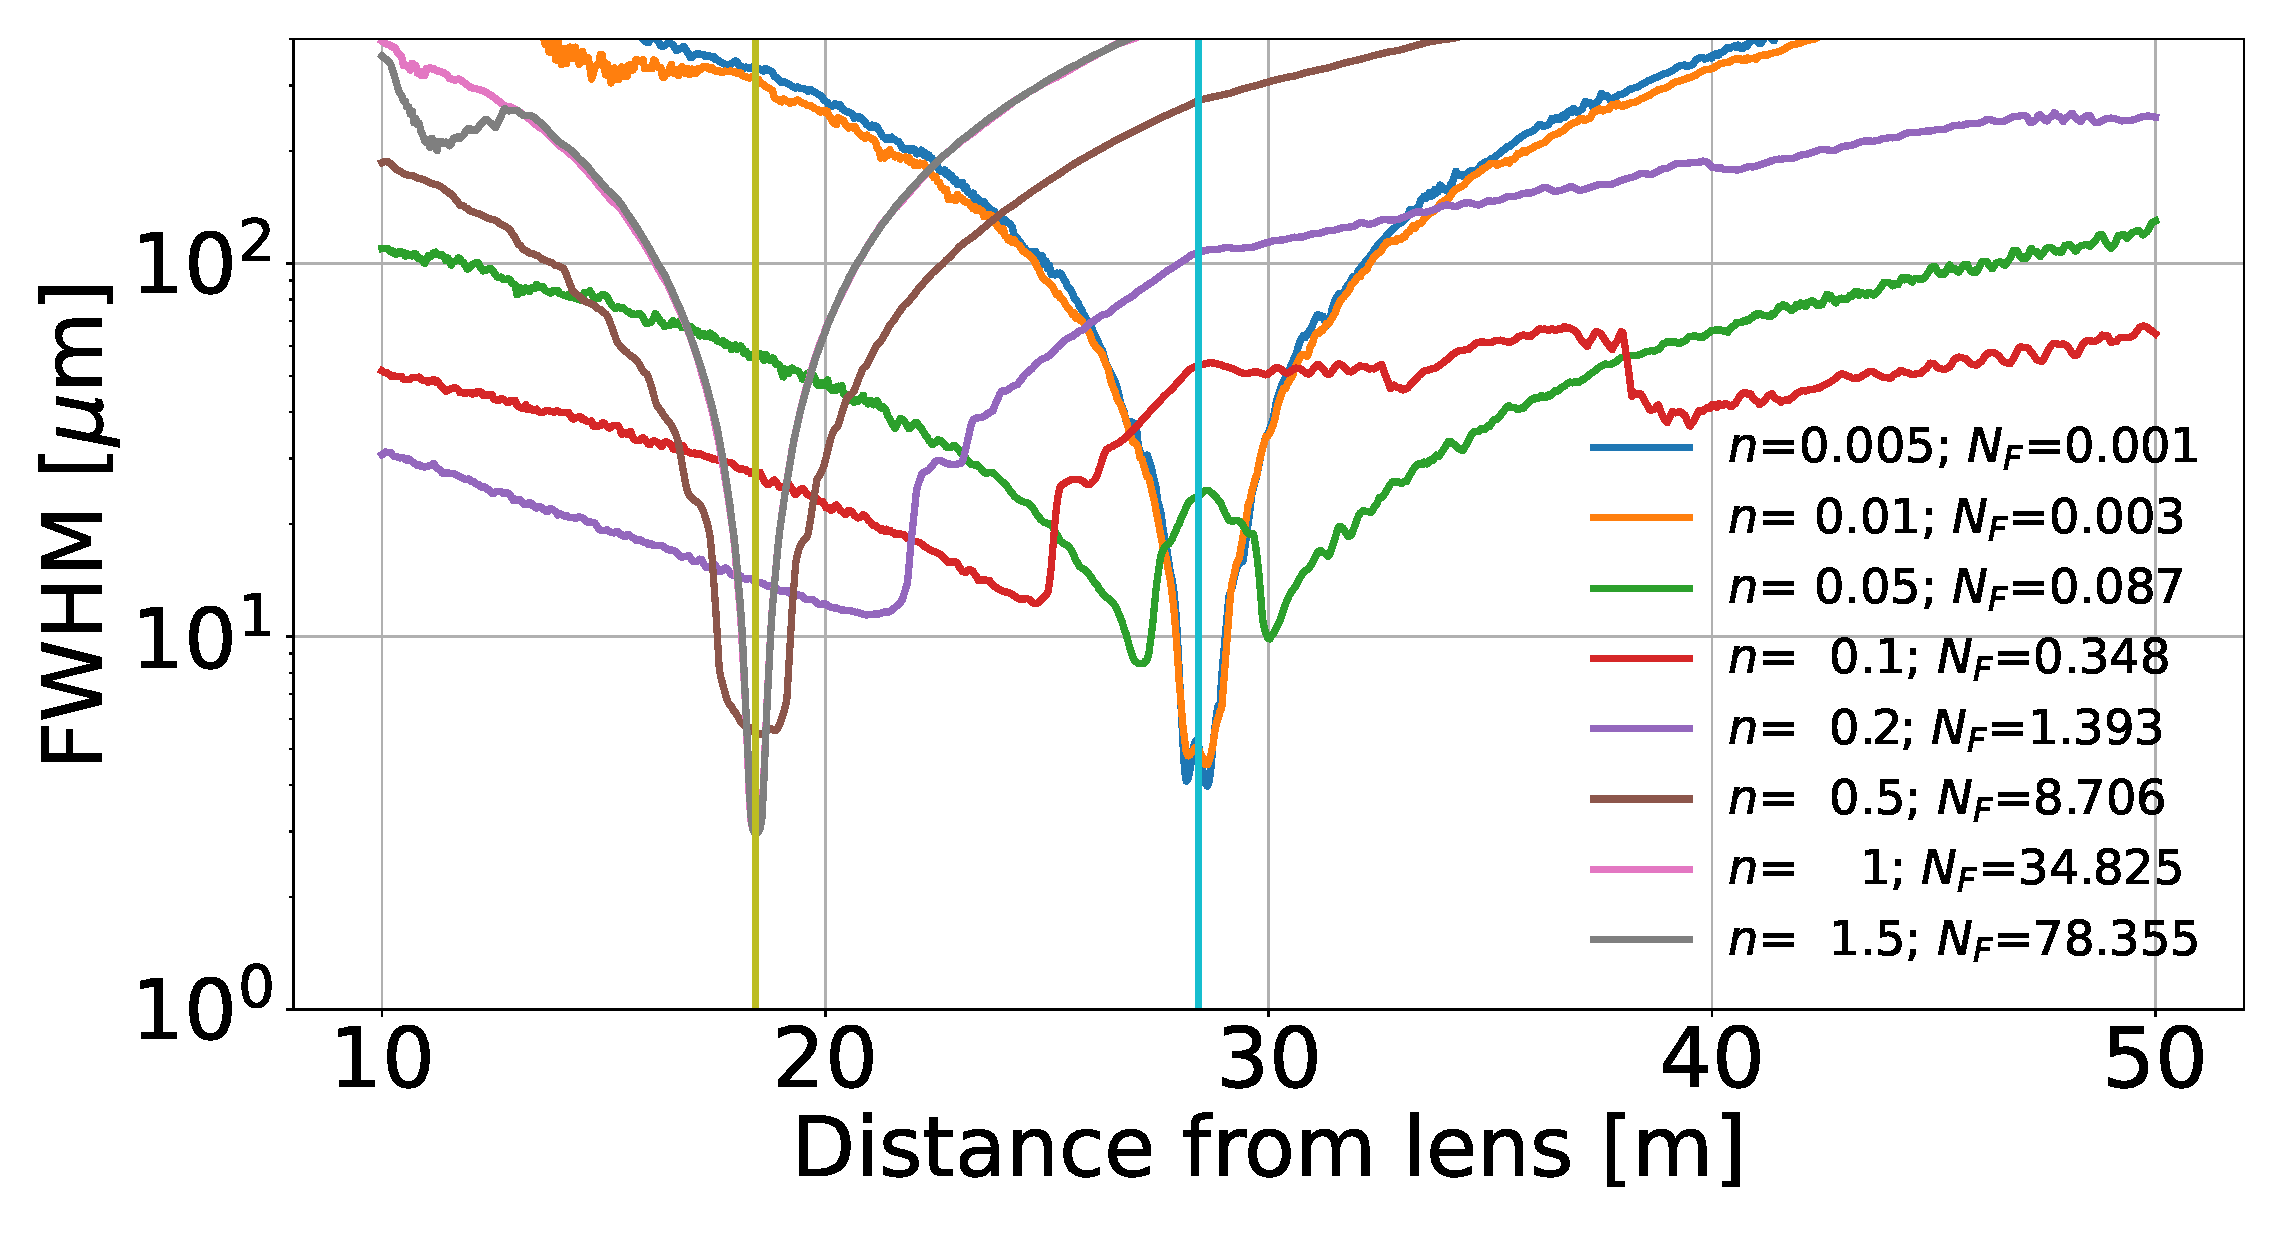
\includegraphics[width=0.95\textwidth]{figures/oneTF_UndSource_RectSlit_R200um.eps}
\caption{Evolution of the size of a coherent undulator beam cropped by a slit and focused by a lens of $R$=~\SI{0.2}{\milli\meter} 
The plot shows the FWHM of the beam  as a function of the distance from the lens. The aperture is open at $a = n \times a_\text{FWHM}$ with different values of $n$ (shown in the legend) and $a_\text{FWHM}$ = \SI{565}{\micro\meter} (the beam FWHM at the aperture plane). The focal positions given by geometrical optics are represented for the source placed wither at the ID position (yellow vertical line) or at the slit position (blue vertical line).
The Fresnel number $N_F$ calculated at the slit plane is also marked in the legend.
}
\end{figure}

Fig.~\ref{fig:oneTFund} shows the evolution of the beam after being focused by the lens. With the open slit the geometrical optics give a focal position $q=$~\SI{18.4168}{\meter} (source at the ID position, distant $p$ from the lens) and $q_a=$~\SI{28.4089}{\meter} (source at slit position, distant $p_a$ from lens). It can be noticed that for $n\ge$~1 (Fresnel number $N_F\ge$~35) the situation does not change with respect the open slit because the cropping by the slit is negligible. For $n=0.5$ ($N_F=8.7$, brown line) the FWHM of the focal size increases and the depth of focus also increases, manifested in a flat depression. For smaller values of $n$ and $N_F$ the minimum shifts to higher distances (e.g., $n=0.1$ red line) and becomes less pronounced. For $n$ = 0.05 (green line), a small beam size is found again close to the $q_a$ position, but it presents a twin minimum due to the interference fringes found in the intensity distributions. Both minima converge to a the $q_a$ position for $n\le$~0.01 (orange line). 

When the focal distance of the lens is reduced (using lenses with smaller radius, or piling several lenses), the $q$ and $q_a$ positions shift to shorter distances, and  $|q-q_a|$ also reduces. They converge to a single position: the lens focal length $q=q_a=f$. This happens when both source-lens and slit-lens distances can be considered at infinite. 

The dimension of the waist can be calculated using geometrical concepts only for the limiting cases of waist at $q$ and $q_a$. For the waist at $q$, the beam size is the source size times its magnification (ratio between lens-waist distance and lens-source distance). Similarly, for the waist at $q_a$, the beam size is the slit aperture times the magnification (now computed as the ratio between lens-waist distance and slit-lens distance). This has been verified numerically (not shown). However, for intermediate slit apertures, where the waist position is in between $q$ and $q_a$, the waist size is different to that predicted by geometric optics.
Indeed, it can be observed in Fig.~\ref{fig:oneTFund} that for these intermediate slit apertures that crop the beam, the waist size is larger than those found at limiting positions $p$ and $p_a$.
This is an important fact: A good focusing, i.e., a very small beam size is only obtained in the limiting cases of open slit and almost-closed slit. This means that for a fully coherent beam, the slit disturbs the focusing and should be avoided. The diffraction at the slit creates an an spurious divergence that affects the lens power. 

The calculation shown in Figure~\ref{fig:oneTFund} refers for the zero emittance case (complete coherence, or $CF_h=CF_v=1$). Next section extends these results to the more realistic case of finite emittance.

\subsubsection{Partial coherence} The mission of the slit is to improve beam coherence (increase coherent fraction). For usual photon energies (5-25~keV)  the slit must be almost closed to gain coherence in old storage rings like ESRF-1 ($CF<10^{-3}$), thus forming a secondary source. For storage rings like EBS, with $CF > 10^{-2}$, the selection of the slit aperture $a$ is crucial: the slit must be closed until the the desired $CF$ is obtained, but not more, because it not only reduces intensity but also deteriorates the focusing. 

\begin{figure}
    \centering
    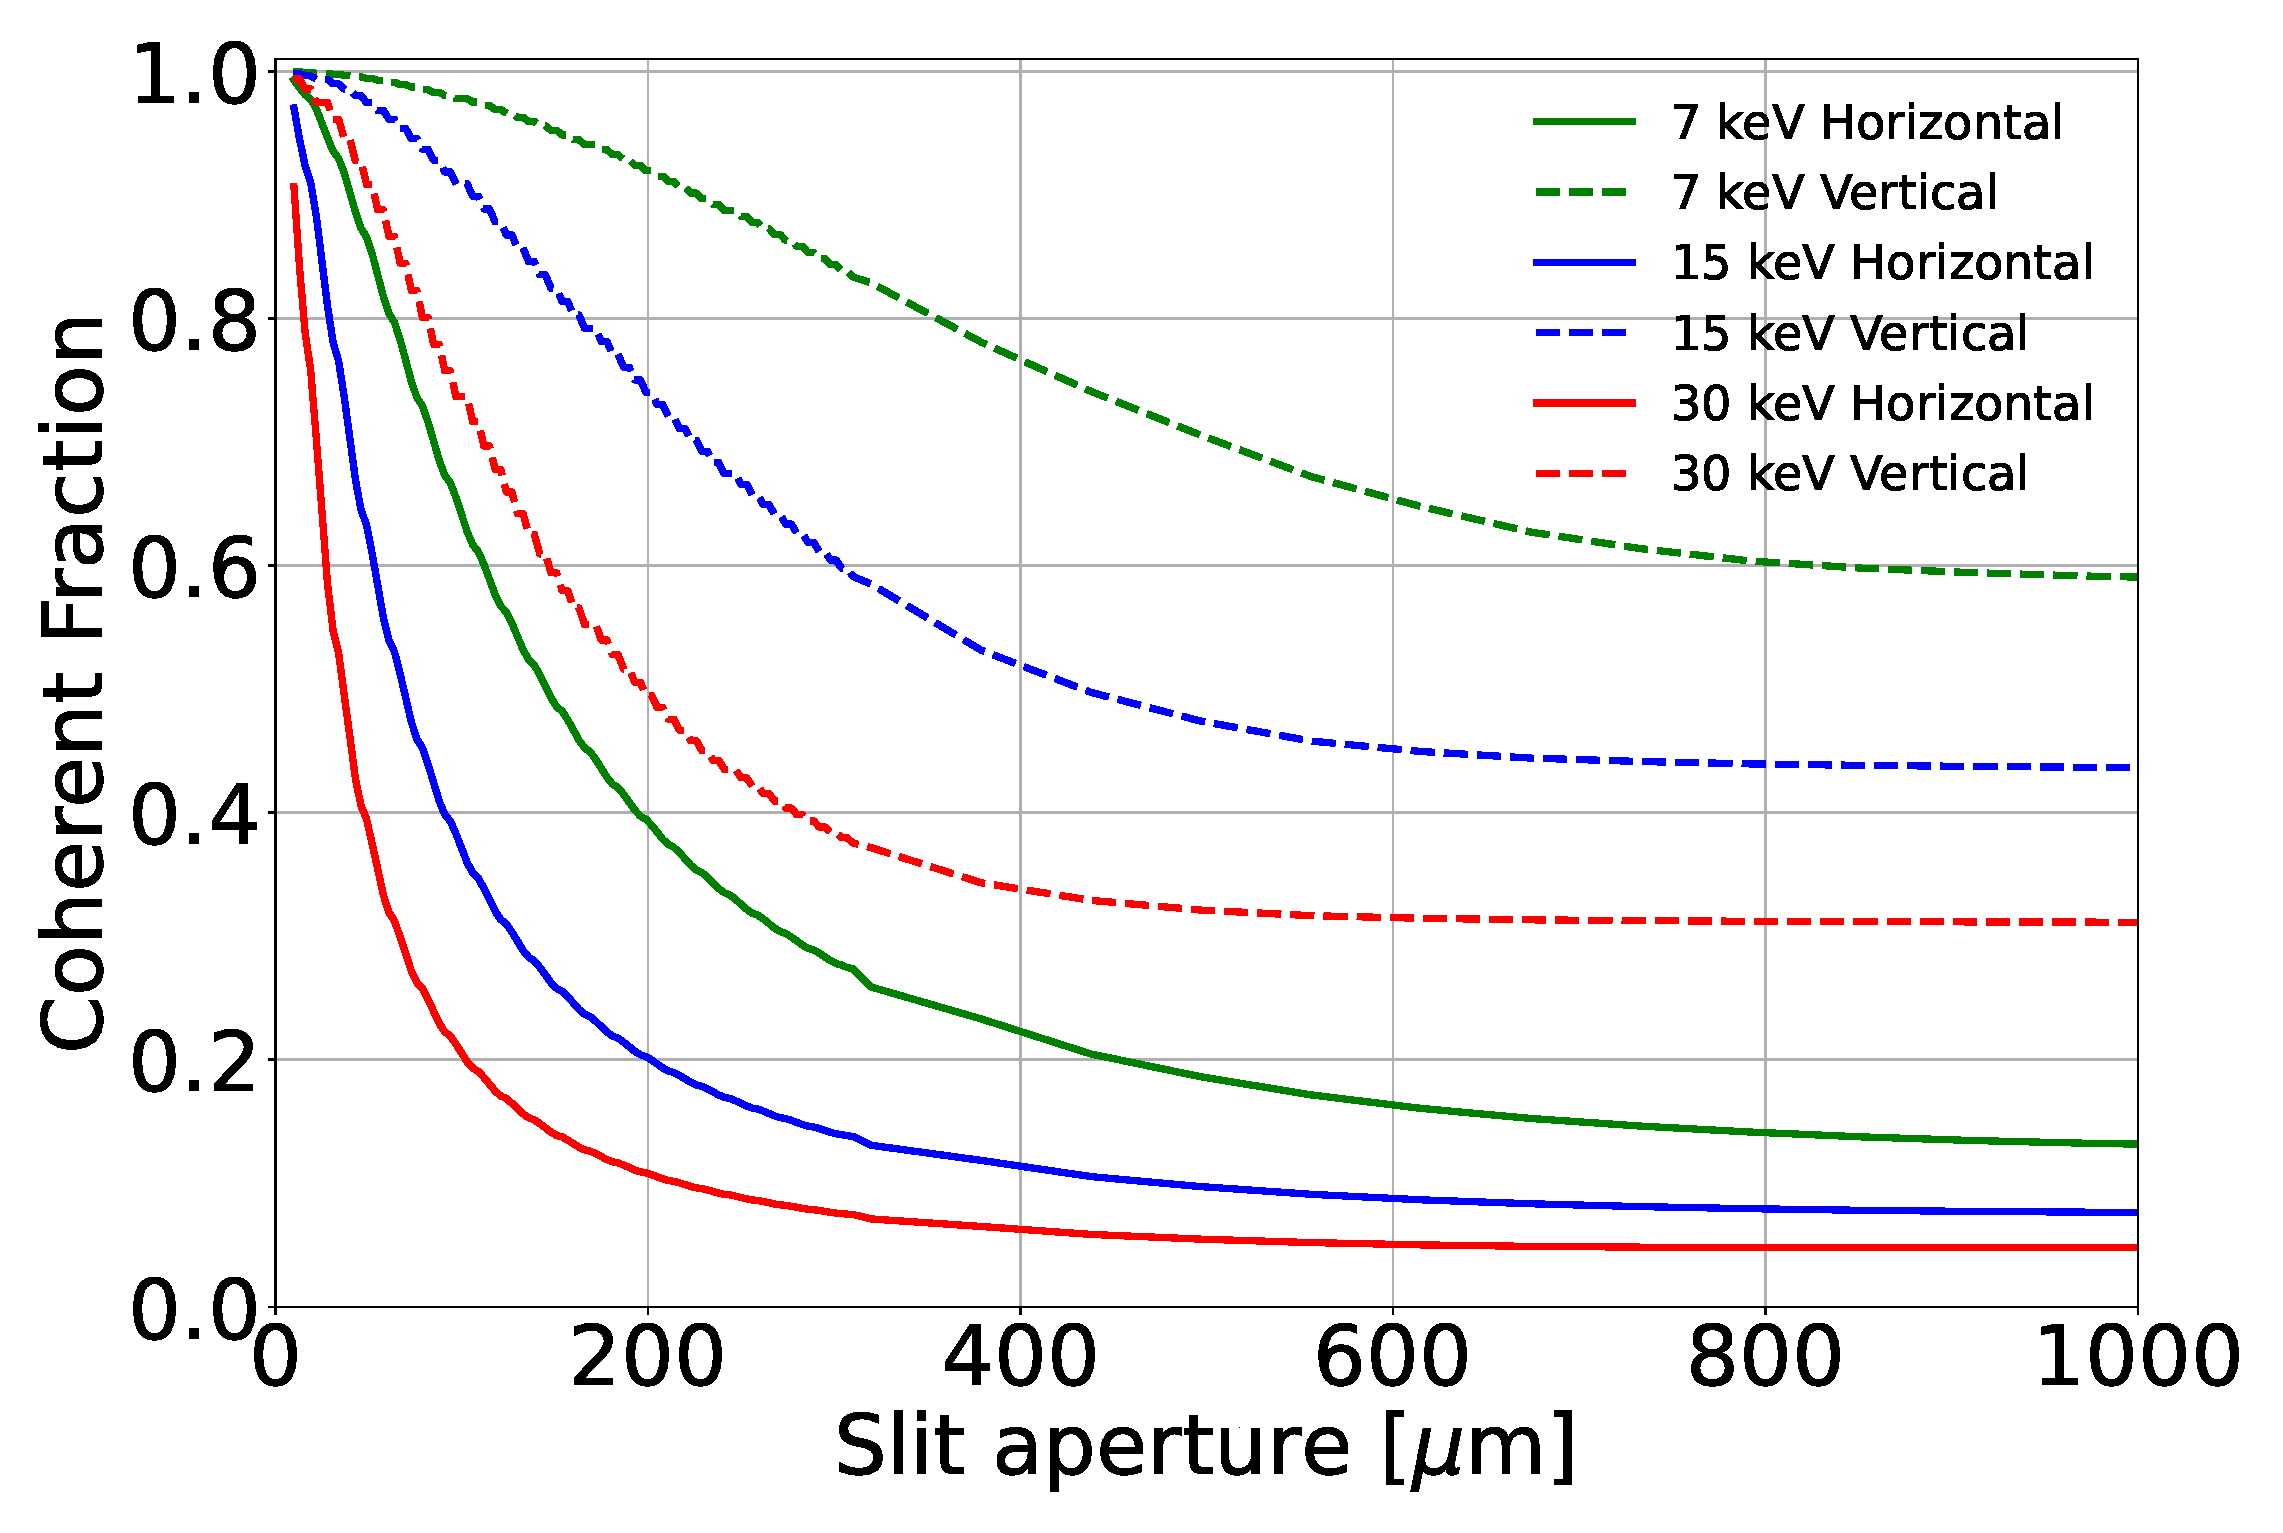
\includegraphics[width=0.95\textwidth]{figures/cf_vs_aperture.eps}

    \caption{
    Coherent fraction in the horizontal and vertical directions for different photon energies as a function of the slit aperture $a$. The slit is placed at \SI{36}{\meter} from the ID. 
    % Top axis shows the $n$ factor as in Fig.~\ref{fig:oneTFund} ($n=565/a$).
    }
    \label{fig:cf_vs_aperture}
\end{figure}

We used the EBS-ESRF emittance values\footnote{We used over this work the following values of electron beam sizes at the center of the straight section: $\sigma_x=~\SI{29.7}{\micro\meter}$,
$\sigma_{x'}=~\SI{4.37}{\micro\radian}$,
$\sigma_y=~\SI{5.29}{\micro\meter}$,
$\sigma_{y'}=~\SI{1.89}{\micro\radian}$, corresponding to beam emittances:  $\epsilon_x=~\SI{130}{\pico\meter \radian}$,
$\epsilon_y=~\SI{10}{\pico\meter \radian}$, and beta functions
$\beta_x=~\SI{6.8}{\meter}$,
$\beta_y=~\SI{2.8}{\meter}$
}
to perform the coherent mode decomposition of the undulator source.
This is done for the horizontal and vertical directions, resulting coherent fractions (at 7 keV) of $CF_h=$13\% and $CF_v=$58\%, for the horizontal and vertical directions. These values are much higher than for the old ESRF-1 source, but still low to justify approximating the beam by a coherent beam. Therefore, we propagated a number of modes large enough to contain more than 99\% of the source intensity (36 modes in H and 8 in V). The illumination at the entrance slit plane is \SI{610}{\micro\meter} in H times \SI{566}{\micro\meter} in V. The slit aperture is used to tune the coherence of the beam: closing the slit increases the $CF$. In the limit (zero aperture) the beam after the slit is fully coherent ($CF=1$), but obviously with zero intensity. The choice of the right slit aperture comes from a compromise between coherence and flux. Figure~\ref{fig:cf_vs_aperture} shows the $CF$ after of the H and V 1D beams after the slit for different slit apertures. From this figure we select the apertures to be used in the following simulations. We selected a photon energy of \SI{7}{keV}. A first value of $CF_h=CF_v=$ 90\% in both horizontal and vertical (thus with a combined 2D  $CF=CF_h CF_v=$ 81\%) is obtained with slit apertures of
$a_h$ =~\SI{40.3}{\micro\meter}, and 
$a_v$ =~\SI{227}{\micro\meter} (horizontal and vertical, respectively). A second value of  $CF_h=CF_v=$ 70\% (thus 2D $CF$ of about 50\%), corresponds to 
$a_h$ =~\SI{85.1}{\milli\meter}, and 
$a_v$ =~\SI{506.7}{\milli\meter}. The case of the ``open" slit that does not crop the beam is also included (this is obtained, for example, with $a_h$ =~\SI{1}{\milli\meter} and $a_v$ =~\SI{1.5}{\milli\meter}).

\begin{figure}\label{fig:oneTFundPartialCoherence}
    \flushleft a) {\it horizontal}\\ \centering
    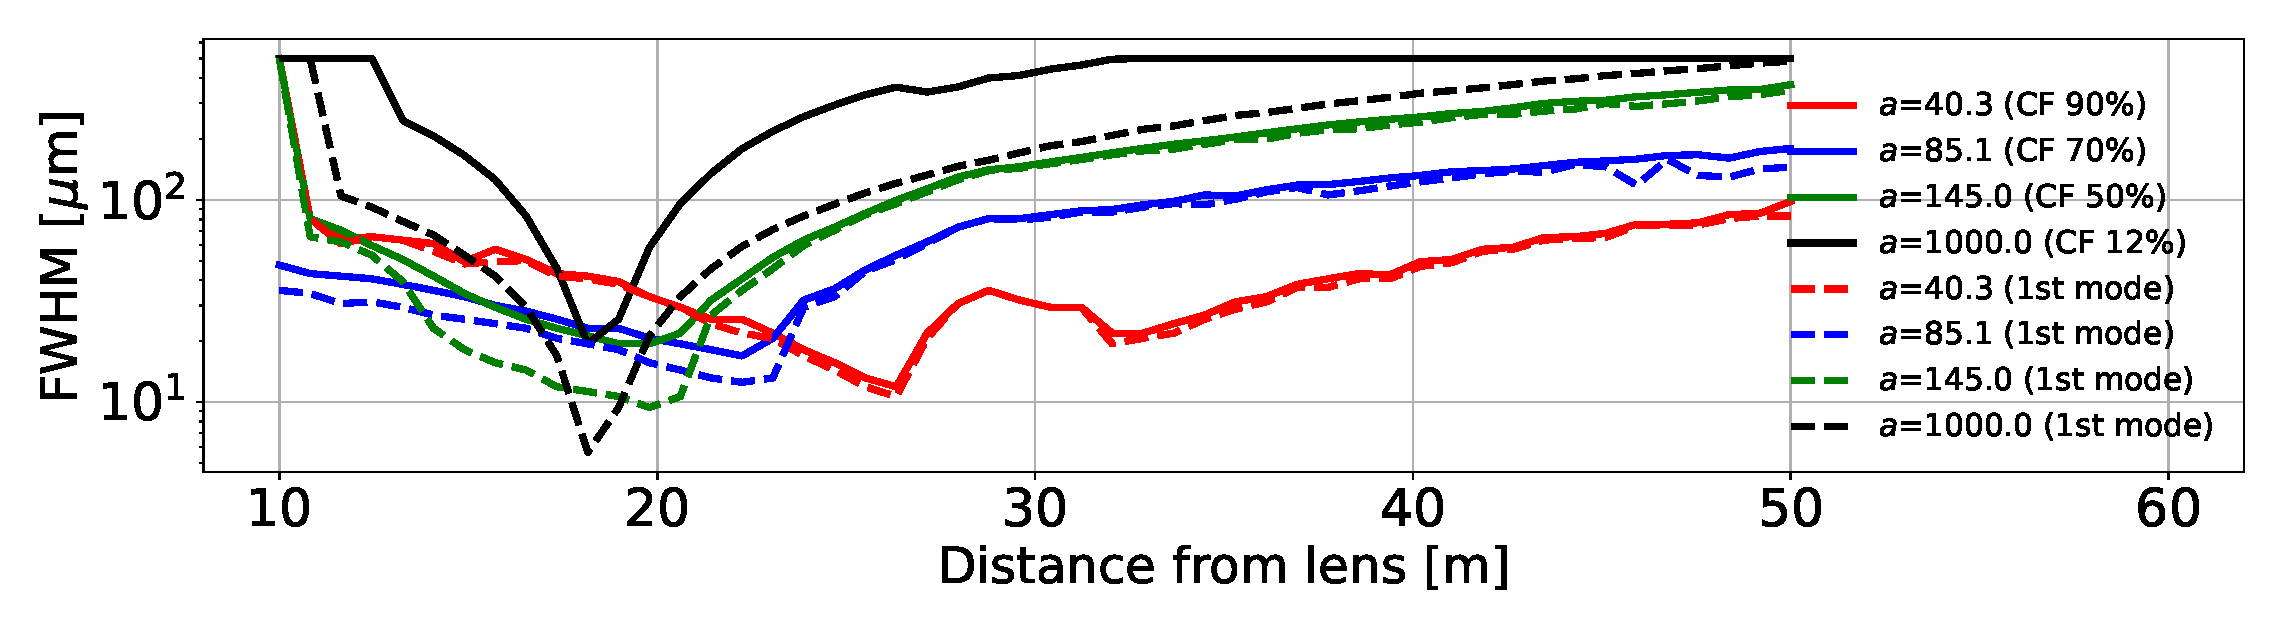
\includegraphics[width=0.95\textwidth]{figures/oneTF_UndSource_RectSlit_R200um_PartialCoherence_h.eps}
    \flushleft b) {\it vertical}\\ \centering
    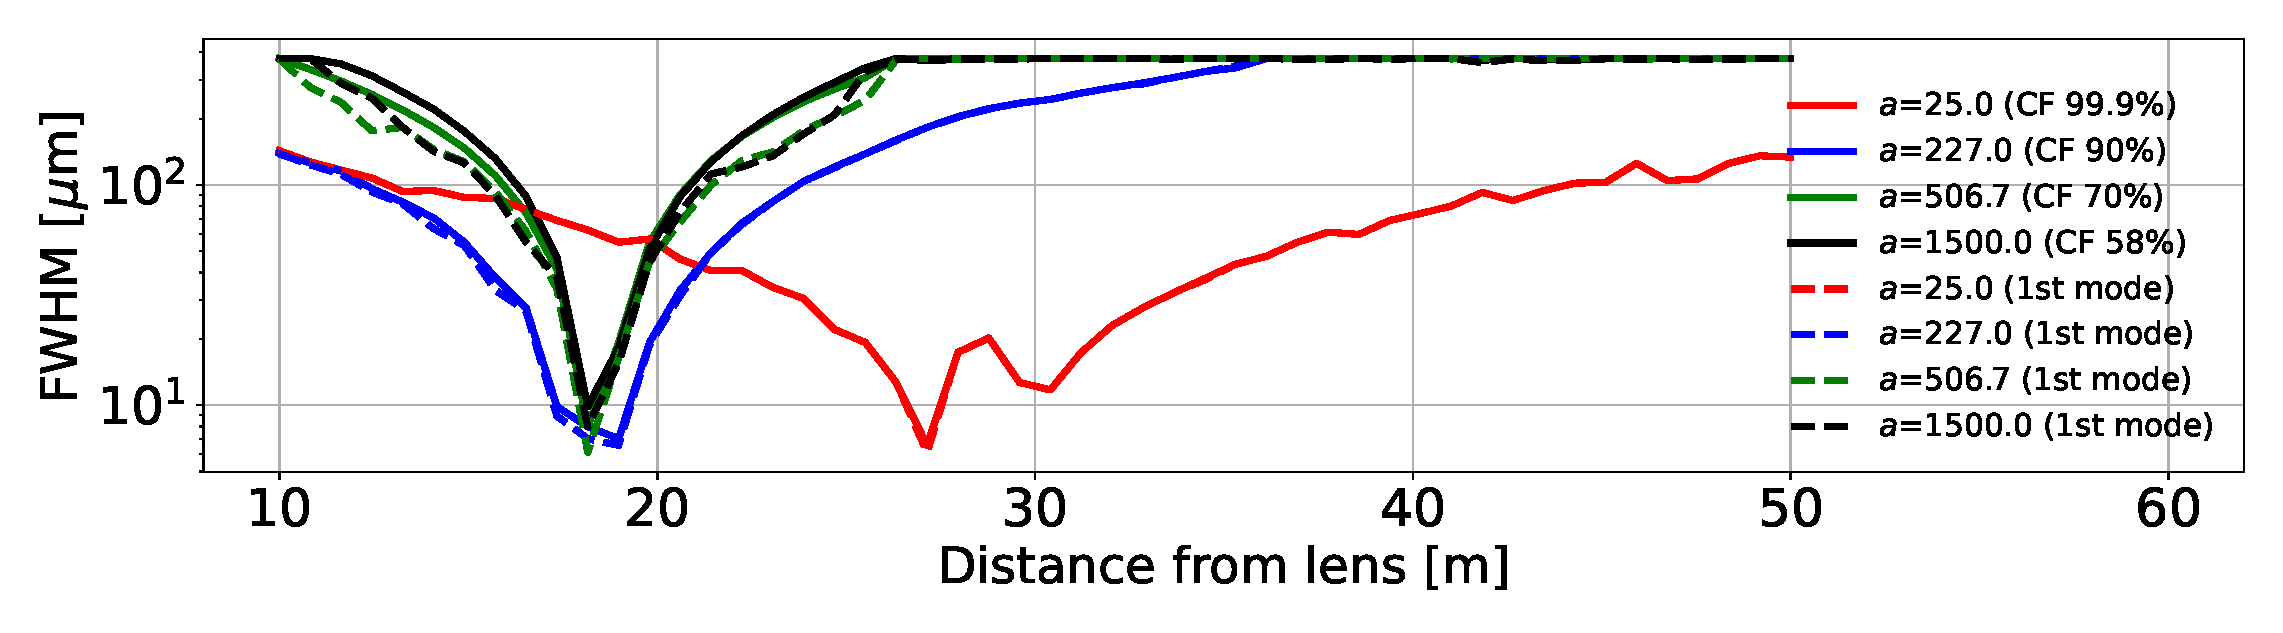
\includegraphics[width=0.95\textwidth]{figures/oneTF_UndSource_RectSlit_R200um_PartialCoherence_v.eps}

    \caption{Evolution of the size of a coherent undulator beam cropped by a slit and focused by a lens of $R$~=~\SI{0.2}{\milli\meter} in the a) horizontal and b) vertical directions.
    The plot shows the FWHM of the beam  as a function of the distance from the lens.
    Full lines correspond to the partial coherent (multimode) beam, whereas the dashed lines correspond to the full coherent beam (first mode). Different slit apertures are used for obtaining different coherent fraction after the slits (marked in legend).
    }
\end{figure}

Figure~\ref{fig:oneTFundPartialCoherence} shows the focal size along the optical axis for these apertures in the horizontal and vertical planes. We calculated the case of the partially coherent beam (multi-mode, solid lines) and also the case of a fully coherent beam (only the first coherent mode, dashed lines). We observe that the focal positions (the minima of the plot lines) do not change significantly when passing from full to partial coherence. However, the focal dimension changes significantly in the horizontal direction for cases with $CF_h\le$ 70\%. In the vertical, where the beam at the source was more coherent there is no differences in sizes when going from full (dashed lines) to partial coherence (solid lines).

Looking to the focal position shift versus slit aperture we find important differences in the horizontal and vertical. The cropping of the beam by the slit is important in horizontal as we need to increase the $CF_h$ from the source (13\%) to values required by the experiments, usually larger than 50\%. This produces a gradual shift of the focal position from the position of the geometrical image of the ID source (black line in panel a)) to the geometrical image of the slit (red line in panel a)). However, in the vertical plane, the slit crops the beam only slightly, and closing the slit to go from the source $CF_v$ = 58\% to values up to 90\% does not produce any focal shift from the position of the geometrical image of the ID source. Only when the slit is very closed (e.g., $a_v$ =~\SI{25}{\micro\meter}, red curve) the focal position shifts to the geometrical image of the slit. This case is in principle not interesting experimentally as it reduces the intensity from an already quite coherent beam ($CF_v$~= 90\%). 

In this section, we have supposed that the 2D beam can be separated in two 1D beams, for H and V directions. No other approximations were made: we used the full undulator source, performed coherent mode decomposition, used an aperture with a rectangular function, and used a Be lens with the real parabolic profile (with thickness $t=$~\SI{50}{\micro\meter} and aperture \SI{1}{\milli\meter}). 

We remarked that hybrid ray-tracing \cite{codeHYBRID} correctly reproduces the effect of shift and degradation of the focal spot when the NA is reduced. The results are shown in Fig.~\ref{fig:oneTF_hybrid}. Compared to Fig.~\ref{fig:oneTFund}, they show a good qualitative agreement (the focal position do agree). This result pushed us to compare our wavefront propagation results with those of hybrid ray-tracing (sections~\ref{sec:complete-beamline} and \ref{sec:discussion}).


\begin{figure}
    \centering
    
    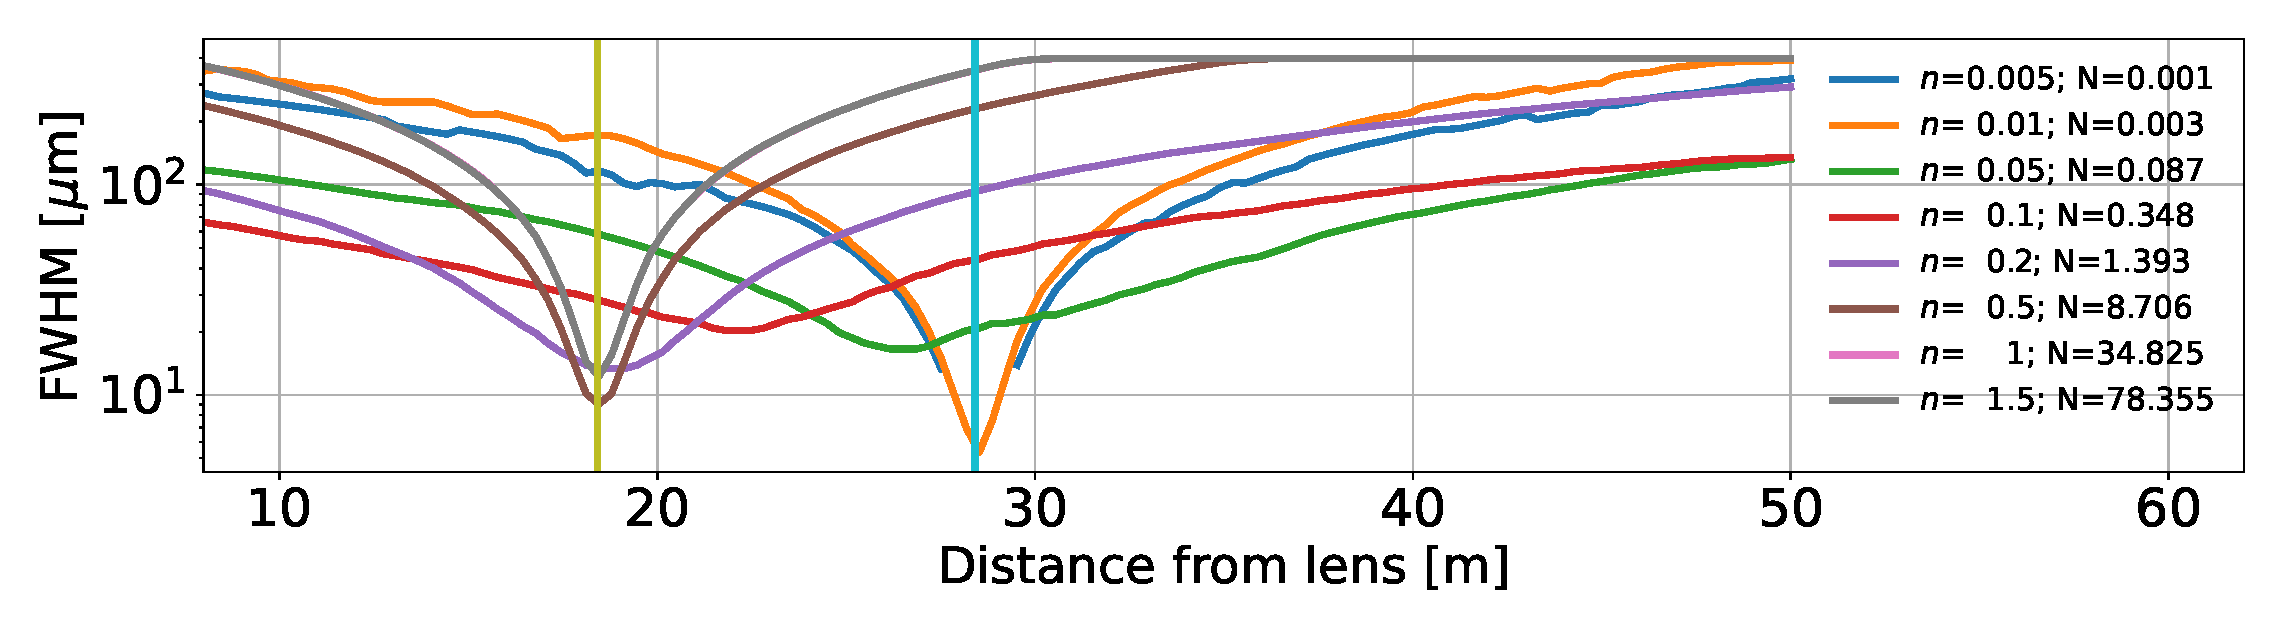
\includegraphics[width=0.95\textwidth]{figures/oneTF_ShadowHybrid_R200um.eps}
    
    \caption{Evolution of the size of a coherent undulator beam cropped by a slit and focused by a lens of $R$~=~\SI{0.2}{\milli\meter} using hybrid ray-tracing.
    }
    \label{fig:oneTF_hybrid}
\end{figure}



\section{Pairing two transfocators}\label{sec:twolenses}

%http://lpc1.clpccd.cc.ca.us/lpc/molander/PDFs/Twolenses.pdf

We study here an optical system composed by two lenses (lens-1 with focal length $f_1$ and lens-2 with $f_2$) separated by a distance $D$. Following \citeasnoun{Goodman85}, the relationship between object-to-lens-1 distance $p_1$ and the lens-2-to-image distance $q_2$ is
\begin{equation}
\label{eq:twolens}
    D-(f_1+f_2)=\frac{f_1^2}{p_1-f_1} + \frac{f_2^2}{q_2-f_2}.
\end{equation}

The global magnification is the product of the magnification of the individual lenses. It can be written as
\begin{equation}
\label{eq:magnification}
    M=M_1 M_2=\frac{1-q_2/f_2}{1-p_1/f_1}.
\end{equation}

The magnification is not dependent on $D$, however the length of the optical system $L=p_1+D+q_2$ will change if one changes the focal distances of the lenses. For a constant $L$ one can change magnification by changing the inter-lenses distance $D$ (zoom effect). In a synchrotron beamline using transfocators, the magnification can be changed by varying the focal lengths of the transfocators (by adding or removing individual or group of lenses in the transfocator) \cite{Vaughan:kv5084}.

We analyze the optical design of a focusing system that uses two transfocators, and how to configure it for the desired focal size or magnification. We start using the oversimplified assumptions of geometrical optics, for then using wave optics simulations with the focusing system illuminated by a partial coherent beam.

\begin{table}[]
    \label{table:id18parameters}
    \caption{Position of the two transfocators, slit and sample (focal point) corresponding to the ID18 beamline configuration under study. }
    \centering
    \begin{tabular}{l|c|c}
         element & position [m] & comment\\
         ID (undulator) source& 0 & U18 $N_u$~=~138 $K$~=~1.851 (7 keV)\\
         Slit & 36 &
         variable aperture $a_h\times a_v$
         \\
         Transfocator 2D & 65 & 
         %$f_H=58.7; f_V=54.3$ 
         \\
         Transfocator 2D & 170 & $D$~=~\SI{105}{\meter} \\
        %  Transfocator 2D & 170 & position 1 {\bf FO1}, $D$=~\SI{105}{\meter} \\
        %  Transfocator 2D & 192 & position 2 {\bf FO2}, $D$=~\SI{127}{\meter}  \\
         sample & 200 & focal plane
    \end{tabular}


\end{table}

The two transfocators in use are idealized as two real beryllium lenses of variable curvature radius $R_1$ and $R_2$ that correspond to focal distances $f_1$ and $f_2$ ($f=R/(2 \delta)$, with $\delta=$~6.96 10$^{-6}$ for Be at \SI{7}{keV}). A slit of aperture $a_h$ in horizontal and $a_v$ in vertical is placed upstream the lens-1. The positions of the elements is determined by room constraints and are considered fixed (although different values could be studied). We set the distances matching the requirements of the EBS-ESRF ID18 beamline (see Table~\ref{table:id18parameters}), and we analyzed the system at a photon energy of \SI{7}{keV}. We study the variation of the spot size as a function of the focal distances. The final goal is to get the desired focal size by selecting the configuration of the transfocators (the focal length and the particular combination of lenses to approach it) . 

\begin{figure}\label{fig:f1f2map}
    \centering

    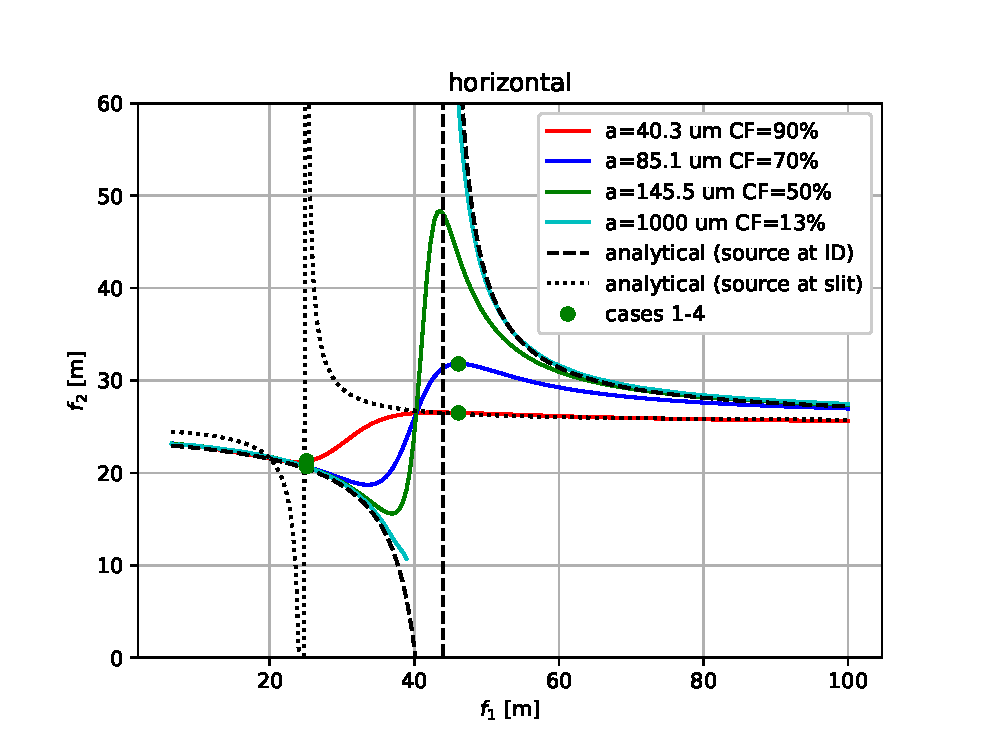
\includegraphics[width=0.95\textwidth]{figures/f1f2_h.eps}
    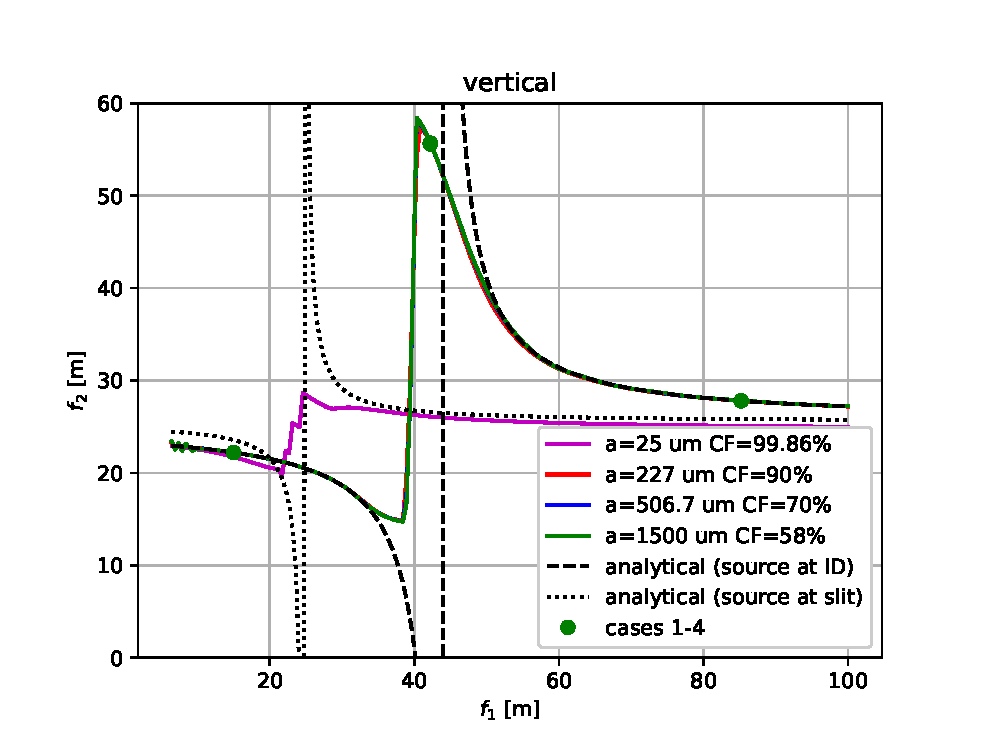
\includegraphics[width=0.95\textwidth]{figures/f1f2_v.eps}

    \caption{Trajectories $(f_1,f_2)$ for $D$~= \SI{105}{\meter} calculated numerically for different values of apertures. Panel a) is for the horizontal direction and panel b) for the vertical. 
    Analytical values displayed are obtained using equation~(\ref{eq:twolens}) with $p_1$~= \SI{65}{\meter} (object at source position) (solid lines) or $p_1$~= \SI{29}{\meter} (object at slit position) (dashed lines).
    }
\end{figure}

For fixed distances $p_1$, $D$ and $q_2$, and also a given value of $f_1$, one can calculate analytically $f_2$ using  equation~(\ref{eq:twolens}) and the corresponding magnification $M$ in the framework of geometrical optics. Taking $f_1$ as variable parameter,  
Fig.~\ref{fig:f1f2map} shows the trajectories of $f_2$ as a function of a variable $f_1$. 
The choice of one pair $(f_1,f_2)$ from these curves guarantees that the focus is at the sample position ($L=p_1+D+q_2$~= \SI{200}{\meter} from source).

Figure~\ref{fig:f1f2map} also shows the value of $f_2$ optimized numerically\footnote{Calculations in this section use a Gaussian slit aperture to minimize diffraction fringes}. 
They are calculated from the analysis of the wavefront phase impinging on lens 2. A correction profile to focus on the sample is calculated using the method described in section~\ref{sec:refractorCorrector}. This profile is fitted with a circle over the central part of the lens, thus giving the radius of curvature or the most adequate lens, and also the its focal length. 
The $(f_1,f_2)$ curves depend strongly on the slit aperture in the horizontal, because of the low $CF_h$ of the source (12\%) is highly increased by the slit. In the vertical the source is more coherent ($CF_v$~=~58\%) therefore the slit improves the $CF_v$  and there is not much change in the trajectories up to values of 90\%. However, in the case of a slit with $a_v$~=~\SI{25}{\micro\meter} that is acting as a pinhole the trajectories (red line) approach the results of the geometrical optics considering the source at the slit position.

\begin{figure}
    \centering
    % \includegraphics[width=0.95\textwidth]{figures/Figure_magnification_99.png}
    %\includegraphics[width=0.95\textwidth]{figures/Figure_magnification_123.png}
    
    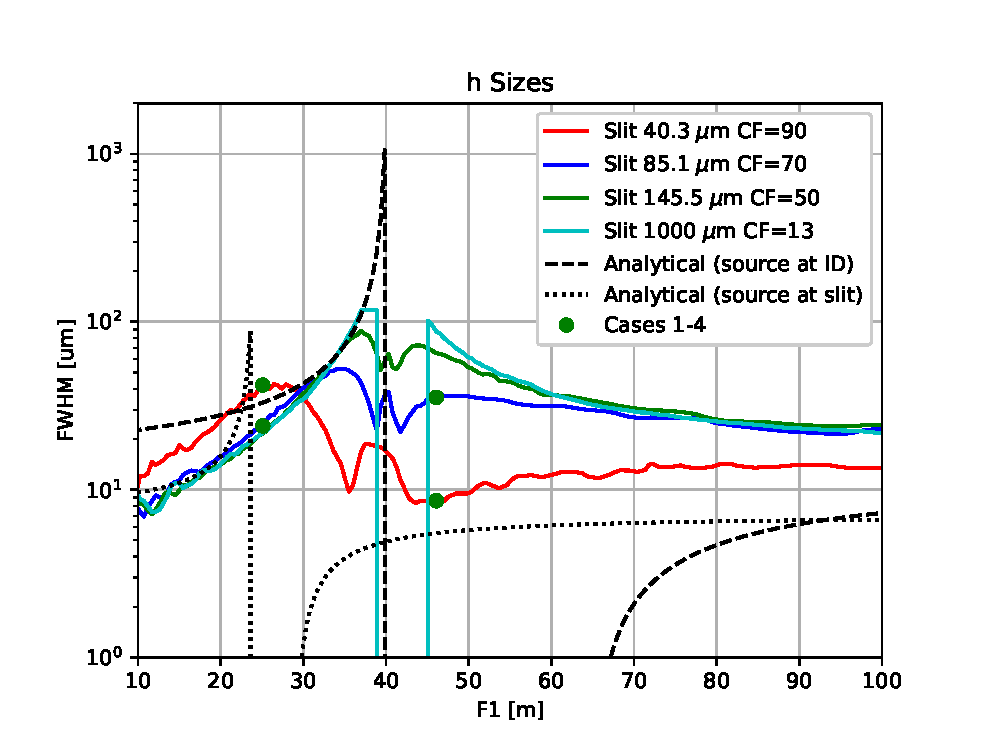
\includegraphics[width=0.95\textwidth]{figures/sizes_h.eps}
    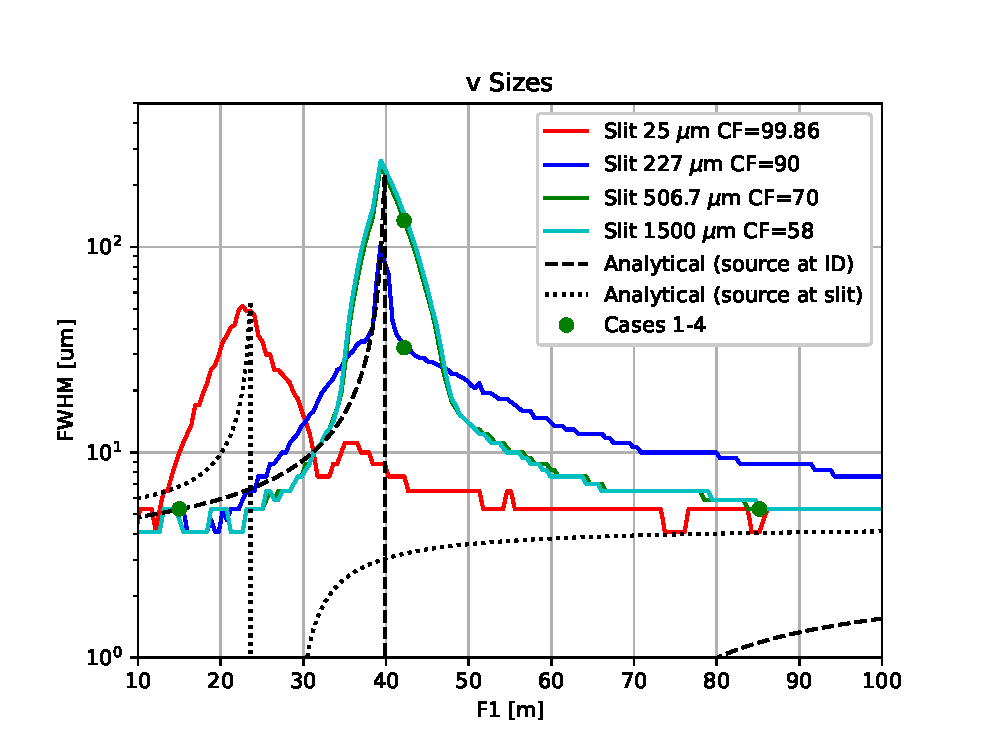
\includegraphics[width=0.95\textwidth]{figures/sizes_v.eps}
        
    \caption{Focal sizes obtained by a two transfocator system as a function of focal length of lens-1 $f_1$. The focal length $f_2$ of the second lens is obtained from the trajectories in Fig.~\ref{fig:f1f2map}. 
    Analytical values are obtained using equation~(\ref{eq:magnification}) with $p_1$~= \SI{65}{\meter} (object at source position) (solid lines) or $p_1$~= \SI{29}{\meter} (object at slit position) (dashed lines). 
    }
    \label{fig:focalSizes}
\end{figure}

Figure~\ref{fig:focalSizes} shows the calculated focal sizes. Analytical values (dashed and dotted lines), based on geometrical optics, use  equation~(\ref{eq:magnification}). They do not reproduce correctly values of beam sizes calculated numerically with wave optics. It can be concluded that the analytical values have very limited applicability, at least in the configurations studied.
In the horizontal direction, for slit apertures $a_h>$~\SI{40}{\micro\meter} the sizes change considerably for small changes in $a_h$. The focusing characteristics of the system depends highly on the diffraction effects produced at the slit. For the slit $a_h$~=~\SI{40.3}{\micro\meter} ($CF_h=$~90\%) the focal size can vary from roughly 10 to 50 microns.  In vertical the focal size can be changed from 5 to 100 \SI{}{\micro\meter} at at $CF_v=$~90\%.


\section{Multiple simulations of the focusing system in the beamline}
\label{sec:complete-beamline}

In this section we analyse particular beamline focusing configurations using several methodologies in detail. We calculate the intensity distribution at the focal plane for four cases. They have been selected from the results in Fig.~\ref{fig:focalSizes}. The first case is selected to obtain a small spot (about \SI{5}{\micro\meter}) and the second one a large spot (more than \SI{30}{\micro\meter}).  For these cases the slits are selected to match a $CF_h=CF_v=$~90\% for a photon energy of \SI{7}{keV}. The values are shown in Table~\ref{table:2Dusercases}. The cases 3 and 4 follow the same logic but the slits are opened to obtain a less coherent beam ($CF_h=CF_v=$~70\%). The analysis is made with different methodologies, using different software codes, following an hierarchical approach, as discussed in \citeasnoun{hierarchical}, with the idea of balancing accuracy and computational effort, to subsequently select and use the most advantageous method for the analyzed problem. This multi-method analysis will also help to validate the new 1D CMD method introduced in this work. The results of the Wofry1D results are compared with other well-known simulation packages. 

\begin{table}[]
    \label{table:2Dusercases}
    \caption{Configurations selected for 2D simulations. Slit aperture ($a_h$ or $a_v$) is selected for obtaining $CF_h=CF_v=$~90\% in cases 1 and 2, and $CF_h=CF_v=$~70\% in cases 3 and 4. Data are obtained from Fig.~\ref{fig:focalSizes}.
    }
    % \centering
    \begin{tabular}{c|c|c|c|c|c|c}
         case h/v & $a_h/a_v$ [\SI{}{\micro\meter}] & $f_1$ [m] & $f_2$ [m] & $R_1$ [\SI{}{\micro\meter}]& $R_2$ [\SI{}{\micro\meter}] & size [\SI{}{\micro\meter}]\\
         \hline
1 h &      40.3 & 46.1 &     26.5 &     641.9 &     369.5 &     8.6 
%&     86
\\
1 v &      227.0 & 15.0 &     22.2 &     209.4 &     309.6 &     5.3 
% & 21
\\
\hline
2 h &      40.3 & 25.1 &     21.3 &     349.1 &     296.3 &     42.0  
% & 42 
\\
2 v &      227.0 & 42.2 &     55.6 &     588.6 &     775.3 &     32.3 
% &     78
\\
\hline \hline
3 h &      85.1 & 46.1 &     31.8 &     641.9 &     443.7 &     35.5 
% &     86 
\\
3 v &      506.7 & 85.2 &     27.8 &     1187.4 &     387.6  &     5.3 
% &     168 
\\
\hline
4 h &      85.1 & 25.1 &     20.7 &     349.1 &     288.7 &     24.0 
% &     42 
\\
4 v &      506.7 & 42.2 &     55.7 &     588.6 &     776.0 &     134.3 
% &     78 

    \end{tabular}
\end{table}

\begin{table}[]
    \label{table:comparison}
    \caption{Comparison of sizes (FWHM, in \SI{}{\micro\meter}) calculated with different methods for the cases defined in Table~\ref{table:2Dusercases}.
    In brackets, the values for the fully coherent beam (single electron with SRW, first coherent mode with COMSYL/WOFRY), and zero emittance with Hybrid).
    }
    \centering
    \begin{tabular}{p{0.05\textwidth}|c|c|c|c|c}
         case h/v &
         Wofry1D&
         COMSYL&
         SRW&
         Hybrid \\
         \hline
1 h  & 8.5(8.1)    & 10.0 (9.9)  & 8.6 (7.5)   & 17.3 (17.5) \\
1 v  & 4.8(4.8)    & 4.7 (5.1)   & 4.6 (4.6)   & 3.3 (3.1) \\
\hline
2 h  & 39.9(38.2)  & 39.5 (39.5) & 40.0 (36.1)  & 39.9 (37.5) \\
2 v  & 32.4(29.6)  & 30.6 (29.3) & 34.4 (29.6)  & 74.0 (75.3) \\
\hline
3 h  & 37.5(29.0)  & 36.6 (28.1) & 40.3 (28.4)  & 43.3 (33.0) \\
3 v  & 6.1 (4.9)   & 6.4 (5.7)   & 6.3 (4.6)    & 6.5 (5.8) \\
\hline
4 h  & 24.6(19.1)  & 26.1 (18.6)  & 27.4 (18.0)   & 27.1 (18.8) \\
4 v  & 133.7(110.3)& 111.7 (90.4) & 137.4 (132.0) & 150.2 (159.8) \
% 1 h  & \inblue{8.6,}8.5(8.1) \inblue{[94]}  & 10.0 (9.9)  & 8.6 (7.5)   & 17.3 (17.5) \\
% 1 v  & \inblue{5.3,}4.8(4.8) \inblue{[97]}   & 4.7 (5.1)   & 4.6 (4.6)   & 3.3 (3.1) \\
% \hline
% 2 h  & \inblue{42.0,}39.9(38.2) \inblue{[94]} & 39.5 (39.5) & 40.0 (36.1)  & 39.9 (37.5) \\
% 2 v  & \inblue{32.3,}32.4(29.6) \inblue{[90]} & 30.6 (29.3) & 34.4 (29.6)  & 74.0 (75.3) \\
% \hline
% 3 h  & \inblue{35.6,}37.5(29.0) \inblue{[77]} & 36.6 (28.1) & 40.3 (28.4)  & 43.3 (33.0) \\
% 3 v  & \inblue{5.3,}6.1 (4.9)  \inblue{[77]} & 6.4 (5.7) & 6.3 (4.6)   & 6.5 (5.8) \\
% \hline
% 4 h  & \inblue{24.0,}24.6(19.1)\inblue{[77]}  & 26.1 (18.6) & 27.4 (18.0)  & 27.1 (18.8) \\
% 4 v  & \inblue{134.4,}133.7(110.3)\inblue{[71]}& 111.7 (90.4) & 137.4 (132.0) & 150.2 (159.8) \\
    \end{tabular}
\end{table}


\subsection{Model WOFRY 1D}
We have recalculated the cases shown in Table~\ref{table:2Dusercases} using Wofry. We optimized manually some parameters, including the zoom factor for propagation in drift spaces. We then combined the 1D horizontal and vertical profiles (using the outer product) to form the 2D intensity profile at the focal plane. Results are shown in Fig.~\ref{fig:2DWofry1D}. We can observe in the intensity distributions a variety of features that are due to the diffraction effects. Case 1 shows an horizontal profile mostly triangular with shoulders that evidence small diffraction fringes. The fringes are more resolved in the vertical direction. Case 2  presents in horizontal a soft Gaussian-like profile, but in vertical important symmetric shoulders are remarked. Case 3 shows a smooth Gaussian profile in horizontal \todo{check/mention the wiggles that are probably artifacts} and a small shoulder with fringes in vertical. Case 4 shows a conventional smooth profile in horizontal but an original three-lobe plateau in vertical. This variety of profile distribution demonstrates how relevant the diffraction effects are, which modulate the beam shape in a non-trivial way.  

\subsection{2D Model COMSYL}
COMSYL performs full CMD of undulator beam \cite{glass2017}. It requires high performance computing (HPC) to solve the Friedholm problem and obtain the full 2D eigenfunctions (coherent modes) and eigenvalues.
Simulation of the source with COMSYL took 55 min using  
28 x 3.30 GHz CPUs of 251.82 GB RAM, for getting 174 modes of 1691 $\times$ 563 pixels.
Once COMSYL calculates the source, OASYS is used to propagate the modes along the beamline.
The propagation uses 2D propagators and optical elements available in Wofry. Results are shown in Fig.~\ref{fig:comsyl}. This figure shows results very similar to Fig.~\ref{fig:2DWofry1D}, which is reasonable because the physical models used for the CMD and propagation are similar. \inred{The beam profiles calculated with COMSYL are a bit more noise, as the number of pixels cannot be as high as in Wofry within a reasonable CPU usage.} \todo{TO BE CHECKED/RECALCULATED} This full calculation with COMSYL helps us to validate the approximation at the basis of the 1D CMD introduced in this work: the 1D CMD for the beamline under study gives essentially the same results as the full 2D CMD with COMSYL.



\subsection{2D Model SRW}
SRW~\cite{codeSRW} is a well-established code in the synchrotron community for simulating the emission of synchrotron sources and propagating it along a full beamline. It can be used in single-electron (SRW-SE) mode, where the source is the fully coherent undulator radiation in an ideal storage ring with zero emittance. To include finite-emittance, and therefore the production and propagation of partial coherent beams, SRW uses the multi-electron (SRW-ME) algorithm, that propagates many wavefronts each one created by an electron that enters in the ID with different initial conditions (position and direction) that are sampled from the parameters of the electron beam (moments or Twiss parameters) using a Monte Carlo method \cite{codeSRW_ME}. This method allows to produce accurate intensity maps (by adding the intensity of individual electrons) and is possible to calculate other parameters of the partially coherent-beam, such as coherence lengths. However, it is not able to store the 4D CSD nor to calculate the CF. The SRW-ME requires the use of HPC. 

We have simulated the cases shown in Table~\ref{table:2Dusercases} using SRW-ME, and results are shown in Fig.~\ref{fig:srw}. We performed a convergence analysis as described in Appendix~\ref{appendix:srw} to determine the minimum number of electrons needed to get accurate results. The SRW-ME simulations for the cases analyzed converge with only a few thousands electrons, that can be run in less than one hour in a node with 28 CPUs totalizing 256 GB. The reason is that the beam after the slit has a relatively high CF. 

The agreement between the results of SRW (Fig.~\ref{fig:srw}) with Wofry1D (Fig.~\ref{fig:2DWofry1D}) is striking. All intensity distributions reproduce exactly the same features, and the FWHM values are different in less than 12\%, a value that is compatible with the errors of the simulations (discussed in section~\ref{sec:discussion}). This results validates, once more, the 1D CMD method proposed here, whose requirements in computer power are extremely low (it runs very fast in an averaged laptop).  

\subsection{2D Model hybrid ray-tracing}
The use of pure ray tracing methods (based in geometrical optics) is not adequate when analyzing optical systems dealing with coherent beams (originating diffraction effects). Conventional ray tracing does not reproduce the effects of focal position shift and focus degradation when the NA is reduced. However, ray tracing-based methods much simple and fast than wave-optics-based methods, and in many occasions they are very useful to evaluate the impact of the beam coherence when studying a synchrotron beamline. Because of that, a hybrid \cite{codeHYBRID} algorithm has been developed, incorporating concepts of coherent diffraction in the ray tracing code SHADOW \cite{codeSHADOW}. It is fully   integrated in the ShadowOUI \cite{codeSHADOWOUI} add-on in OASYS. It has been demonstrated to be an efficient and fast tool to design beamlines also including coherence effects. The hybrid ray-tracing can reproduce the effect of degradation of the focus shift and focal shift when changing the NA, as shown in Fig.~\ref{fig:oneTF_hybrid}. 

We analysed the four cases defined in Table~\ref{table:2Dusercases} with hybrid ray tracing.  Figure~\ref{fig:hybrid} displays the results.  One can observe that the intensity distributions are no so rich, in the sense that  features obtained with full wave-optics methods (like the three-lobe plateau in case 4v are not reproduced. However, values of FWHM are close to full wave-optics calculations for most cases, with the exception of two particular cases:
1h (hybrid \SI{16.5}{\micro\meter} Wofry1D \SI{8.5}{\micro\meter}),
2v (\SI{71.2}{\micro\meter} Wofry1D \SI{32.4}{\micro\meter}). They will be discussed in the next section.

\newpage

\begin{figure}\label{fig:2DWofry1D}
    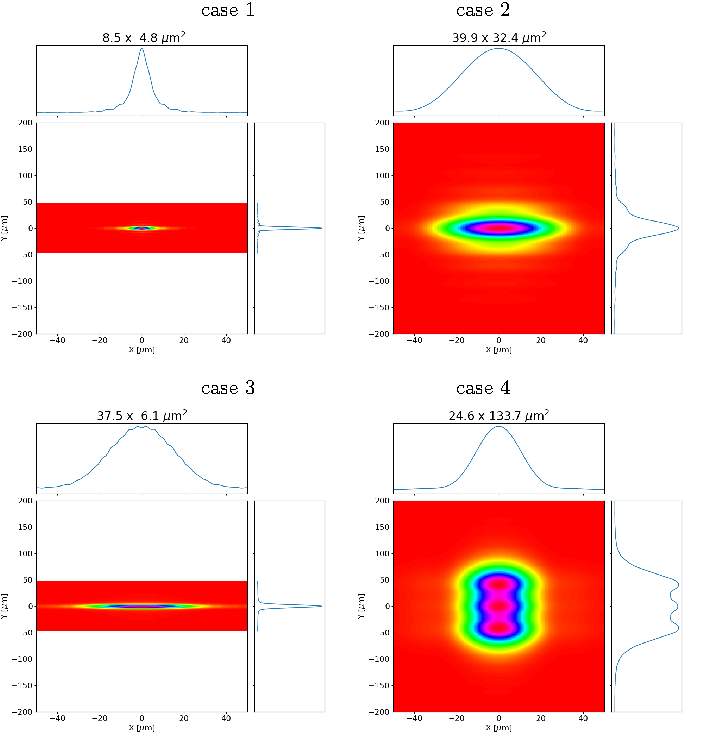
\includegraphics[width=0.99\textwidth]{figures/fig_wofry.pdf}
    \caption{2D intensity distribution at the focal plane. It has been constructed from the Wofry1D calculations.
    \todo{Group all these four figures in a single one}
    }
\end{figure}

\begin{figure}\label{fig:comsyl}
    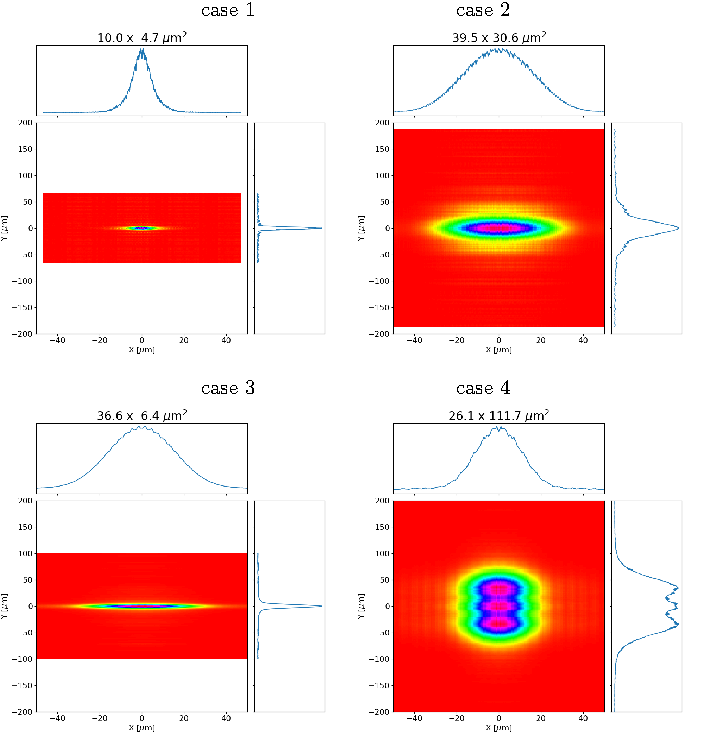
\includegraphics[width=0.99\textwidth]{figures/fig_comsyl.pdf}
    \caption{COMSYL calculations of the intensity distribution at the focal plane for the cases listed in Table~\ref{table:2Dusercases}.
    }
\end{figure}

\begin{figure}\label{fig:srw}
    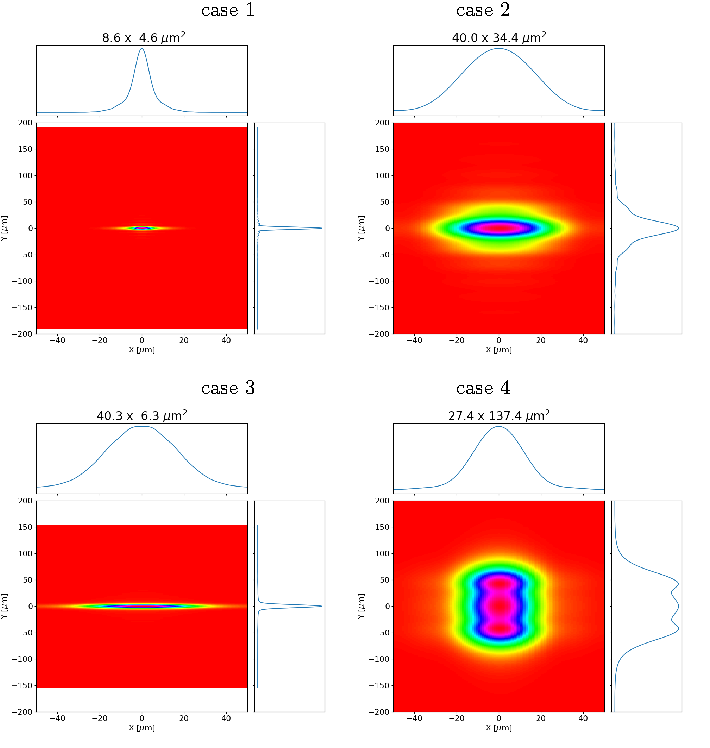
\includegraphics[width=0.99\textwidth]{figures/fig_srw.pdf}
    \caption{Multi-electron SRW calculations of the intensity distribution at the focal plane for the cases listed in Table~\ref{table:2Dusercases}.}
\end{figure}

\vspace{1cm}

\begin{figure}
    \label{fig:hybrid}
    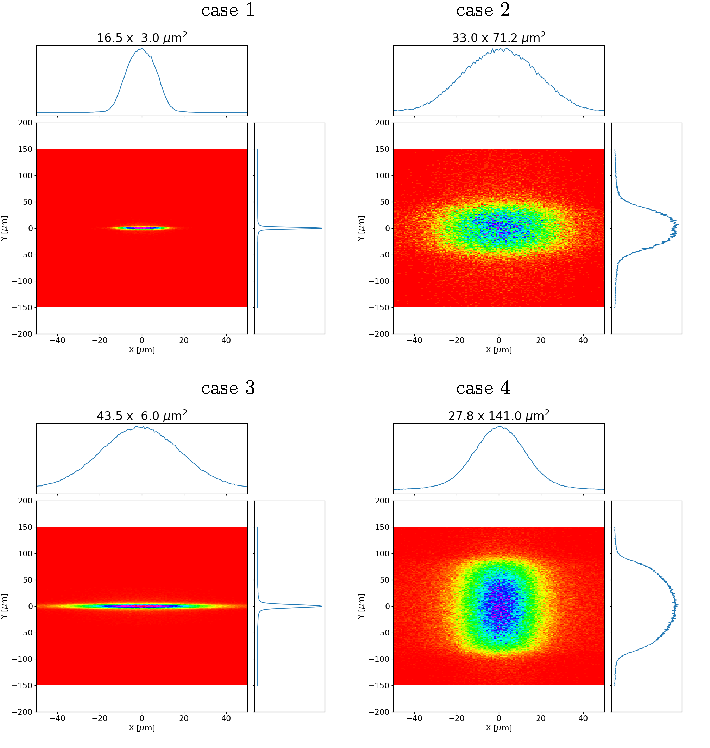
\includegraphics[width=0.99\textwidth]{figures/fig_hybrid.pdf}
    \caption{Hybrid ray tracing calculations of the intensity distribution at the focal plane for the cases listed in Table~\ref{table:2Dusercases}.}
\end{figure}


\newpage


\section{Discussion}
\label{sec:discussion}


\subsection{$f_1$ $f_2$ trajectories and focal sizes} 

The focusing of the partial coherence x-ray beams produced by low emittance storage rings is a complex phenomenon, because diffraction effects induced by coherence modify significantly the  beam characteristics. The concepts of geometrical optics often used to calculate the focal position (lens equation) and the focal size (using magnification) fail when the x-ray beam is cropped significantly (reduced NA) (see Figs.~\ref{fig:f1f2map}, \ref{fig:focalSizes}).
The system studied here, based on the project for the new ID18 beamline at EBS-ESRF, will image directly the source to the focal plane (sample), using two focusing elements (paired transfocators). This is an innovative concept only possible thanks to the high coherence that the new storage rings provide. Beamlines in old synchrotrons always imaged the source into a secondary source at least in horizontal. The use of a secondary source is advantageous in terms of controlling the size with a slit and therefore the coherence, but the drastic reduction in distance source-sample reduces the benefits of the long beamlines. Also, bringing the source closer to the sample imply a larger beam divergence that affects negatively to the transmittivity. Transmittivity depends on the optical element acceptance, usually limited by the extremely good surface finish required. Indeed, in most nonofocusing beamlines (e.g. the ID16A beamline at ESRF \cite{ID16A, hierarchical}) the focal size is mainly defined by  the aperture which also limits the transmittivity to values close to the coherent fraction. At the ID18 beamline at the EBS-ESRF source, the goal is obtain a variable beam size, but keeping flux as high as possible. It is therefore driven by the requirements on coherence controlled by the slit. Imaging the source directly on the sample is much affected by the NA and beam coherence, as our results show. Note also that the ID18 will be able to work in other configurations not analyzed here, giving higher demagnification (with the transfocator 2 closer to the sample). It will also be possible to use a secondary source, the image of transfocator 1, placed close before transfocator 2.

For the EBS-ESRF, the horizontal coherent fraction is lower than the vertical one (Fig.~\ref{fig:cf_vs_aperture}). This implies the necessity of cropping the beam more horizontally than vertically to get $CF_h=CF_v$, thus the smaller NA induces more distortions in the beam. In the vertical direction, the beam must be less cropped, causing smaller beam distortion than in horizontal direction. The horizontal apertures used to obtain typical values of CF suitable for experiments (50-95 \%) do strongly affect the evolution of the beam, but are not small enough to consider the slit as a secondary source. This is manifested in the shift and degradation of the focus that the first transfocator creates (Fig.~\ref{fig:oneTFund}): whereas in vertical most of the typical apertures (down to \SI{227}{\micro\meter}) induce the optical system to image the source (at the ID center), in horizontal the slit aperture required to obtain $CF_h=$ 90\% provokes a "shifting" of the source from its real position (ID center) to the slit position. Although this shift of the focal position has been predicted and calculated before (see \citeasnoun{Tanaka:85} for Gaussian beams, or \citeasnoun{westfahl} for synchrotron beams) our calculations in Fig. 3 reveal two new facts: i) the shift exists but it is directed upstream to the position defined by the geometrical optics for the slit image (and not downstream to the lens position, as found for the systems analyzed in the references mentioned), and ii) the focal size is highly degraded (its size increases) when the beam focus is found in between the two positions defined by the geometrical optics.  

Pairing two transfocators consists in matching their focal distances to guarantee the focus at the desired focal plane (the sample position). By matching the lens equations of the two lenses, it is possible the analytical expression in Eq.~\ref{eq:twolens} permits to calculate $f_2$ as a function of $f_1$. This can be done for the two cases: with the source at the ID center (limit of high NA, no cropping) of with the source at the slit (pinhole limit when NA~$\rightarrow$~0). The analytical equations diverge at the position where lens-1 focuses onto lens-2.
Figure~\ref{fig:f1f2map} shows an asymptotic approach (for $f_1<$~\SI{25}{\meter} or $f_1>$~\SI{70}{\meter}) of the numerical results to geometrical optics results, mostly with source at the ID, but sometimes (with closed slit) to the case of the source at the slit position. However, this case is obtained in the horizontal direction with a reasonable aperture $a=$~\SI{40.4}{\micro\meter} (to reach good coherence $CF_h=$~90\%) but with a very small aperture in the vertical direction $a=$~\SI{25}{\micro\meter}, a less interesting setup because high coherence can be obtained with more opened slits without compromising transmission. 

Equation~\ref{eq:CMD} predicts analytical singularities in $f_2$ when lens-1 focuses on lens-2. The numerical results (Fig.~\ref{fig:f1f2map}) show smooth transition from one branch to another, softer for smaller NAs in the horizontal (Fig.~\ref{fig:f1f2map}a) but not relevant in the vertical (Fig.~\ref{fig:f1f2map}b). As NA is reduced, the inflexion point shifts from the position calculated with the source at the center of the ID to the source at the slit position. However, as discussed in the last paragraph, this shifting is evident in the horizontal for the usual slit openings, but is not yet relevant in vertical for common apertures. 

It is remarkable that the focal sizes calculated in Fig.~\ref{fig:focalSizes} differs considerably from the results of the geometrical optics, making it not adequate to estimate focal sizes using geometrical concepts driven by source demagnification. Only in some particular areas geometrical optics give good results: in horizontal around $f_1\approx$~\SI{30}{\meter}, and at  $f_1 <$~\SI{30}{\meter} in vertical. 

In summary, the numerical simulation of the $(f_1,f_2)$ trajectory maps present two characteristics: i) they asymptotically match the analytical positions for sufficiently high or small $f_1$, either the position obtained when the source is at ID (high NA) or when the source is at the slit (low NA), and ii) the analytical singularities found when lens-1 focuses on lens-2 are smoothed originating an inflexion point that shifts, when reducing the NA, from the analytical position considering the source at the center of the ID to the position with the source sitting at the slit.   
 

\subsection{Methods of calculation}

The results presented here in Fig.~5 contain more than one thousand individual simulation (2 directions $\times$ 4 slits $\times$ 200 points in $f_1$). Each point in the graph represents a calculation including full partial coherence simulations that involves the transport of many modes. This has only be possible with the development of a new fast Wofry1D code for coherent mode decomposition method outlined in Section~\ref{sec:theory}. The results from the some selected configurations in Section~\ref{sec:complete-beamline} (Figs.~\ref{fig:f1f2map} and \ref{fig:focalSizes}) validate the accuracy of the Wofry1D method by comparing its results with full 2D methods (COMSYL and SRW). The wave optics simulations using the three methods (Wofry1D, COMSYL and SRW) give very similar results. 
There is good agreement in focal size FWHM values \todo{(discrepancies less that 10-15\%??)}, but also in the shape of intensity distributions (compare Figs. ~\ref{fig:2DWofry1D}, ~\ref{fig:comsyl} and ~\ref{fig:srw}). The Wofry1D code can be run in a few seconds in a laptop, whereas the simulation of the full CMD with COMSYL required about 1h (for 1691 x 563 pixels, 174 modes) using 1 node of 28 cores. This source is then reused for propagating the different configurations. Each configuration required a full SRW-ME with 5000 electrons run in also about 1h in a similar configuration. 

The specific numeric value for sizes calculated with the different methods (Table~\ref{table:comparison}) depends not only on the code itself, but also on the particular specific parameters in each method (number of pixels for sampling wavefronts, propagation parameters, etc.). To estimate the calculation error in the final size numbers, we vary randomly these specific parameters in a reasonable range (e.g., 10\%). The evaluation of the mean size and the dispersion (standard deviation) of the sizes obtained give an good estimation of the error in this parameter. This exercise would take a considerable computational effort using 2D methods, but it can be easily done with Wofry1D. We run 200 cases with 10\% random variation in the values in number of pixels and magnification factor in drift spaces. The obtained sizes (horizontal $\times$ vertical) are  
8.49 $\pm$ 0.60 $\times$ 4.97 $\pm$ 0.37 \SI{}{\micro\meter}$^2$ (case 1),
39.94 $\pm$ 2.98 $\times$ 32.77 $\pm$ 2.69 \SI{}{\micro\meter}$^2$ (case 2),
36.39 $\pm$ 2.89 $\times$ 6.12 $\pm$ 0.51 \SI{}{\micro\meter}$^2$ (case 3), and
24.18 $\pm$ 1.80 $\times$ 133.44 $\pm$ 10.06 \SI{}{\micro\meter}$^2$ (case 4). We confirmed that the values given in Fig.~\ref{fig:2DWofry1D} are within these error intervals.

\subsection{Hybrid ray tracing}

The simulation results for the four cases studied using the hybrid method indicate that, although this method does not reproduce exactly the intensity distibution given by full partial coherent optics, the numerical values are approaching the good ones, but with two exceptions: the case 
1h (hybrid \SI{16.5}{\micro\meter} Wofry1D \SI{8.5}{\micro\meter}) and the case 
2v (\SI{71.2}{\micro\meter} Wofry1D \SI{32.4}{\micro\meter}). 
We remark that these thee cases have in common that the $f_1$ value in use is close to $f_1$~=~\SI{40}{\meter} that corresponds to the singularity in the analytical (geometrical optics) calculations, when the lens-1 focuses on lens-2. A detailed study with hybrid was performed to calculate the FWHM for all possible values of $f_1$ (as done in Fig.~\ref{fig:focalSizes}. The result (Fig.~\ref{fig:focalSizes_hybrid}) confirms that there is good agreement everywhere except in the region close to $f_1$~=~\SI{40}{\micro\meter}.  \todo{This discrepancy can be originated by... THINK ABOUT THAT...}. We thus conclude that the hybrid ray tracing is a valid method to obtain good values of focal sizes in most cases, excepts for the case that lens-1 focus is close to the position of lens-2 ($f_1 \approx $~\SI{40}{\meter}).
% The hybrid ray tracing reproduces correctly the change in size when changing the $(f_1,f_2)$ pairs (Fig.~\ref{fig:focalSizes_hybrid}). However, we found some differences in the shape of the some intensity profiles, with less marked diffraction fringes, thus manifesting less correct treatment of the fringes evolution. 

\begin{figure}
    \centering

    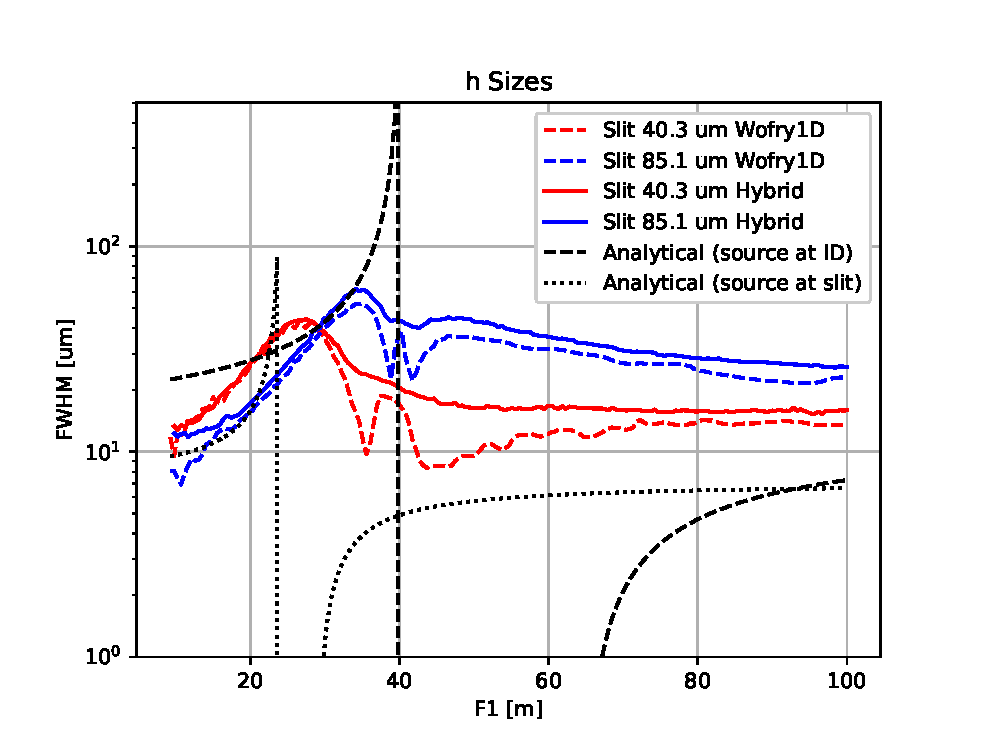
\includegraphics[width=0.95\textwidth]{figures/sizes_h_hybrid.eps}
    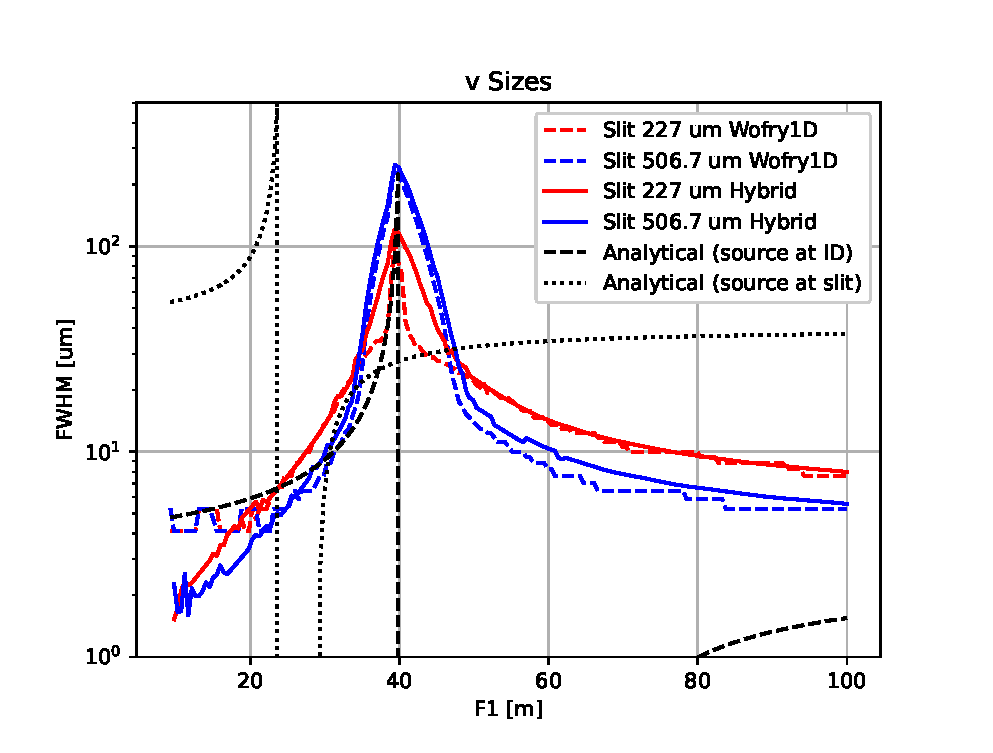
\includegraphics[width=0.95\textwidth]{figures/sizes_v_hybrid.eps}
        
    \caption{Focal sizes obtained by hybrid ray tracing method, for two slit aperture cases, compared with values from Wofry1D  (from Fig.~\ref{fig:focalSizes}).}
    \label{fig:focalSizes_hybrid}
\end{figure}

% \subsection{Further simulations}

% The simulations presented here are motivated by the ID18 project but the optical layout has been simplified to the minimum necessary to study the effect of pairing two transfocators. A more complete study including the other optical elements, other transfocator configurations will be presented elsewhere, also for different energies and implementing the effect of surface errors due to thermal load and surface finish. It is however interesting to briefly mention here some results of this study to give a more complete vision of other relevant parameters to consider.

\subsection{Transmitted flux.} We have limited our study to the focal sizes, but it can be complemented with focal flux. At \SI{7}{keV}, the undulator in the configuration selected emits a flux of 1.5 10$^{15}$ photons/s/0.1\%bw. Each of the three elements studied (slit, lens -1 and lens-2) absorb part of the flux. The estimation of the absorption by the slit can be done using simple geometrical arguments, and the absorption by the slits depend on the average Be thickness presented to the beam. The linear attenuation coefficient of Be at 7 keV is $\mu=$~\SI{3}{\centi\meter$^{-1}$}, giving 1.45\% attenuation for a \SI{50}{\micro\meter} thick layer (like lens thickness used in simulations\footnote{In the simulations the horizontal and vertical focusing are separated in two lenses, with accumulated thickness \SI{100}{\micro\meter} thus absorption 3\%}). For the case 1 simulations we extracted the absorption for the different absorbing elements (slit, lens-1 and lens-2) in the case of partial coherence and also for full coherence (see Table~\ref{table:absorption}).

There is excellent agreement for partial coherence. For full coherence, the Wofry1D results are different than the SRW+Hybrid, because the geometry of the 1st coherent mode used to represent the full coherent beam is not the same as the geometry of the filament beam (used in SRW and Hybrid). We note a high absorption in lens-2, due to the fact that in this case the lens-2 is overilluminated, therefore the \SI{1}{\milli\meter} physical aperture absorbs considerably the beam.


% WOFRY1D
% CASE 1 FULL COH Absorption slit, lens1, lens2 : 87.0, 7.6, 48.3 
% CASE 1 PARTIAL COH Absorption slit, lens1, lens2 : 97.6, 7.9, 50.7 
% CASE 2 FULL COH Absorption slit, lens1, lens2 : 87.0, 6.7, 3.8 
% CASE 2 PARTIAL COH Absorption slit, lens1, lens2 : 97.6, 7.0, 3.9 

% CASE 3 FULL COH Absorption slit, lens1, lens2 : 55.9, 5.4, 17.1 
% CASE 3 PARTIAL COH Absorption slit, lens1, lens2 : 89.5, 6.3, 23.4 
% CASE 4 FULL COH Absorption slit, lens1, lens2 : 55.9, 6.8, 3.6 
% CASE 4 PARTIAL COH Absorption slit, lens1, lens2 : 89.5, 8.0, 3.8 

\begin{table}[]
    \label{table:absorption}
    \caption{Comparison of beam intensity attenuation in percent by the slit, lens-1 and lens-2 for the partial coherent beam, 
    % coherent beam (first coherent mode in Wofry1D, filament beam in SRW, zero emittance in Hybrid) and for the partial coherent beam,
    for the four cases studied.
    The Wofry1D data shown here comes after combining the horizontal and vertical wavefronts using the outer product. 
    }
    \centering
\begin{tabular}{l|lll|lll|lll}
case & \multicolumn{3}{c|}{slit} & \multicolumn{3}{c|}{lens-1} & \multicolumn{3}{c|}{lens-2} \\
\hline
     & \rot{Wofry1D} & \rot{SRW} & \rot{Hybrid}
     & \rot{Wofry1D} & \rot{SRW} & \rot{Hybrid}
     & \rot{Wofry1D} & \rot{SRW} & \rot{Hybrid}
\\
\hline
%    &          &      &        &          &      &         &          &       &         \\
%1      &   87.0   & 96.6 & 96.7   & 7.6      & 7.4  & 5.2     & 48.3     & 51.3  & 53.0   \\
1       &   97.6   & 97.6 & 97.2   & 7.9      & 7.6  & 5.2     & 50.7     & 51.1  & 52.6   \\
% 2c    &   87.0   & 96.6 & 96.7   & 6.7      & 6.4  & 4.3     & 3.8      & 3.7   & 3.3    \\
2       &   97.6   & 97.6 & 97.2   & 7.0      & 6.6  & 4.3     & 3.9      & 3.7   & 3.3    \\
% 3c    &   55.9   & 86.0 & 85.6   & 5.4      & 6.11 & 4.7     & 17.1     & 22.7  & 26.6   \\
3       &   89.5   & 90.2 & 88.6   & 6.3      & 6.1  & 4.6     & 23.4     & 21.8  & 25.2   \\
% 4c    &   55.9   & 86.0 & 85.6   & 6.8      & 7.73 & 6.4     & 3.6      & 3.6   & 3.6    \\
4       &   89.5   & 90.2 & 88.6   & 8.0      & 7.7  & 6.2     & 3.8      & 3.6  & 3.6   \\
\end{tabular}
\end{table}
    

% \begin{table}[]
%     \label{table:absorptionOLD}
%     \caption{Comparison of beam intensity attenuation in percent by the slit, lens-1 and lens-2 for the coherent beam (first coherent mode in Wofry1D, filament beam in SRW, zero emittance in Hybrid) and for the partial coherent beam.
%     The Wofry1D data shown here comes after combining the horizontal and vertical wavefronts using the outer product. 
%     \todo{remove this table? Or, complete it with the other cases? It is just for checking...}
%     }
%     \centering
    
%     \begin{tabular}{c|c|c|c|c}
% case  & 
% coherence &
% Wofry1D & 
% % COMSYL & 
% SRW  & 
% Hybrid \\
% 1   &  full &
% % no after-lens slit 87.0, 5.4, 18.8 &
% 87.0, 7.6, 48.3 &
% % 84.8,6.1,22.6  & 
% 96.6, 7.4, 51.3 & 
% 96.7, 5.2, 53.0 \\
% 1     &  partial &
% % no after-lens slit \inblue{97.6,  5.6 , 51.9}
% 97.6,  7.9 , 50.7 &
% %  & 
% 97.6,  7.6 , 51.0  &
% 97.2, 5.2, 52.6\\
% 2     &  full & 
% 87.0, 4.6, 5.5  & 
% % 84.8,4.9,3.4  &
% 96.6,6.4,3.7 &
% 96.7, 4.3, 3.3 \\
% 3     &  full & 
% 55.9, 4.4, 9.7 & 
% % 52.7,4.2,9.6 & 
% 86.0,6.11,22.7 &
% 85.6, 4.7, 26.6 \\
% 4     &  full & 
% 55.9, 5.8, 4.6 & 
% % 52.7,5.5,3.6 &
% 86.0,7.73,3.6 &
% 85.6, 6.4, 3.6
%     \end{tabular}
% \end{table}

\subsection{Accuracy of the focal position and depth of focus}
\label{sec:caustic}

We have calculated the beam evolution in the neighbourhood of the sample position for the four cases studied (see Fig.~\ref{fig:caustic}). From these plots one can obtain the position of the best focus and the depth of focus.

It can be observed sometimes a mismatch between the position of the best focus and its expected position (the sample position, at the zero abscissas). This is due to an error in the calculations of $f_2$ and may have several origins, which are interesting to discuss. 

For pairing two transfocators, the algorithm chosen to calculate the $f_2$ value consist in analyzing the wavefront at the lens-2 position, find a corrector refractive object that would transform the incoming wavefront in a cylindrically convergent wavefront (see section \ref{sec:refractorCorrector}), and fit the radius at the center. We then get the $R_2$ and therefore the $f_2$ value. In addition, to obtain smooth $(f_1,f_2)$ curves in Fig.~\ref{fig:f1f2map} we have used a Gaussian slit (see section \ref{sec:gaussianslit}). This smears out the diffraction fringes, because in an ideallized system where a point source is focused at the sample position, the recorded intensity would correspond to the diffraction pattern of the slit, that can be considered as an "object" placed in the beam (see e.g. \cite{paganin_book}). The use of a Gaussian object implies that its diffraction pattern is a Gaussian with no diffraction fringes. 

For some cases (1h, 1v, 3h) in Fig.~\ref{fig:caustic} there is a quite good agreement between the focal position obtained from the maximum of intensity on-axis (plotted at the top of the image) and our expected position (the zero in the plots). In some other cases (2v, 3h, 4h) the agreement is acceptable, taking into account that the depth of focus can be quite large (of the order of meters). A small correction in $f_2$ would bring the best focus to its ideal position. This correction is necessary because we used a Gaussian slit for calculating the $(f_1,f_2)$ curves and we neglected some oscillations around the curves shown that appear if no Gaussian apodization were done. There are two pathological cases where the algorithm used to calculate $f_2$ did not succeed: the cases 2h and 4v.
The $f_2$ error in 2h is also due to the oscillations in the $(f_1,f_2)$ and can be corrected, as shown in Fig.~\ref{fig:causticcorrection}. However, case 4v cannot be corrected because we would need a divergent lens to bring the focus of $f_1$ to the sample position \todo{check}. Setting $R_2=f_2=\infty$ would reduce the beam size at the sample position, but cannot get the best focus there. However, an ad-hoc defined refractive corrector in the place of lens-2 would do the job.  

The depth of focus change from XX to XX...





\begin{figure}\label{fig:caustic}
\centering

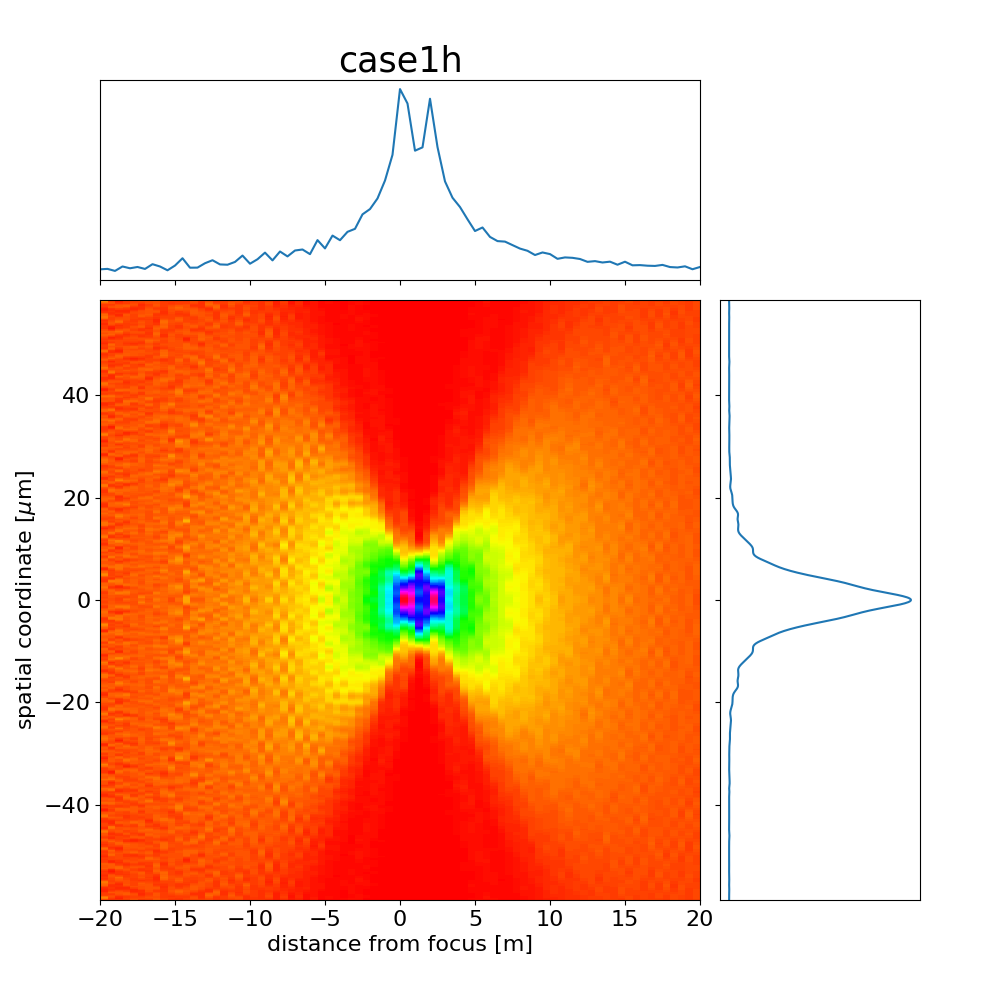
\includegraphics[width=0.49\textwidth]{figures/case1h_caustic.png}
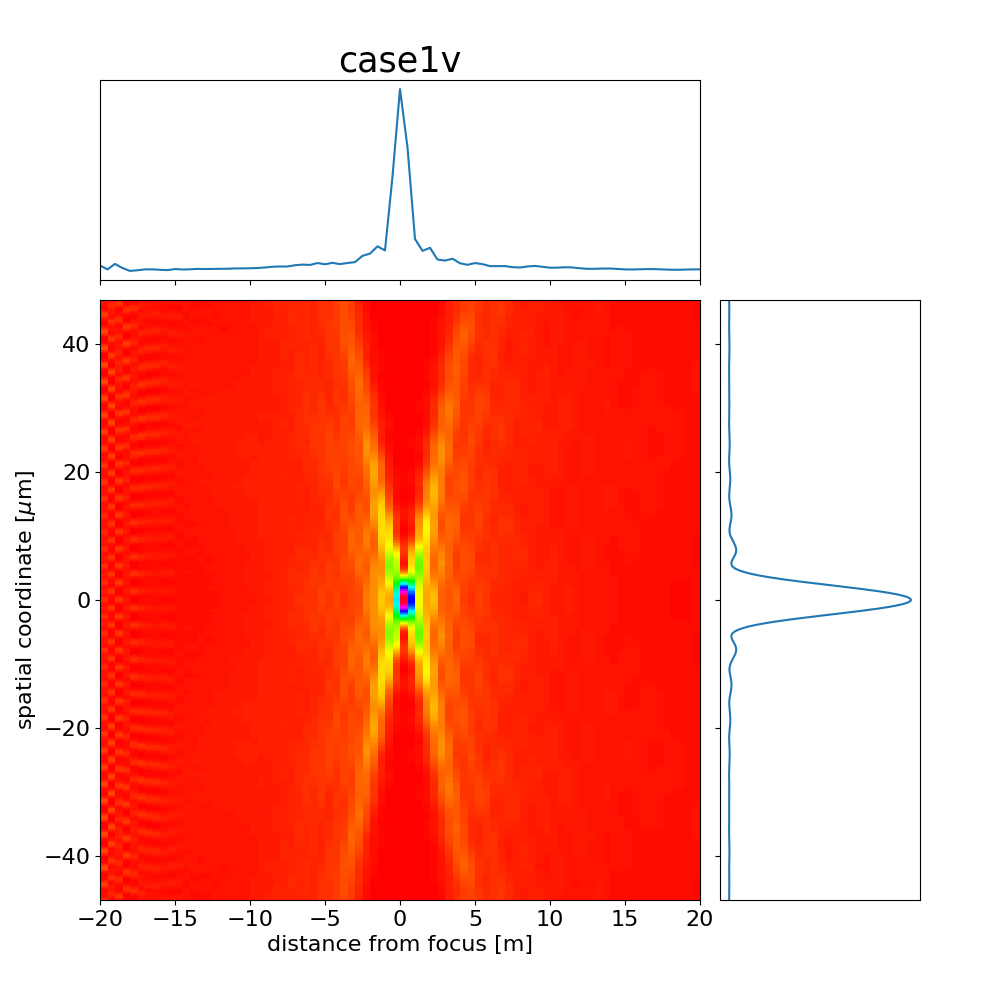
\includegraphics[width=0.49\textwidth]{figures/case1v_caustic.png}

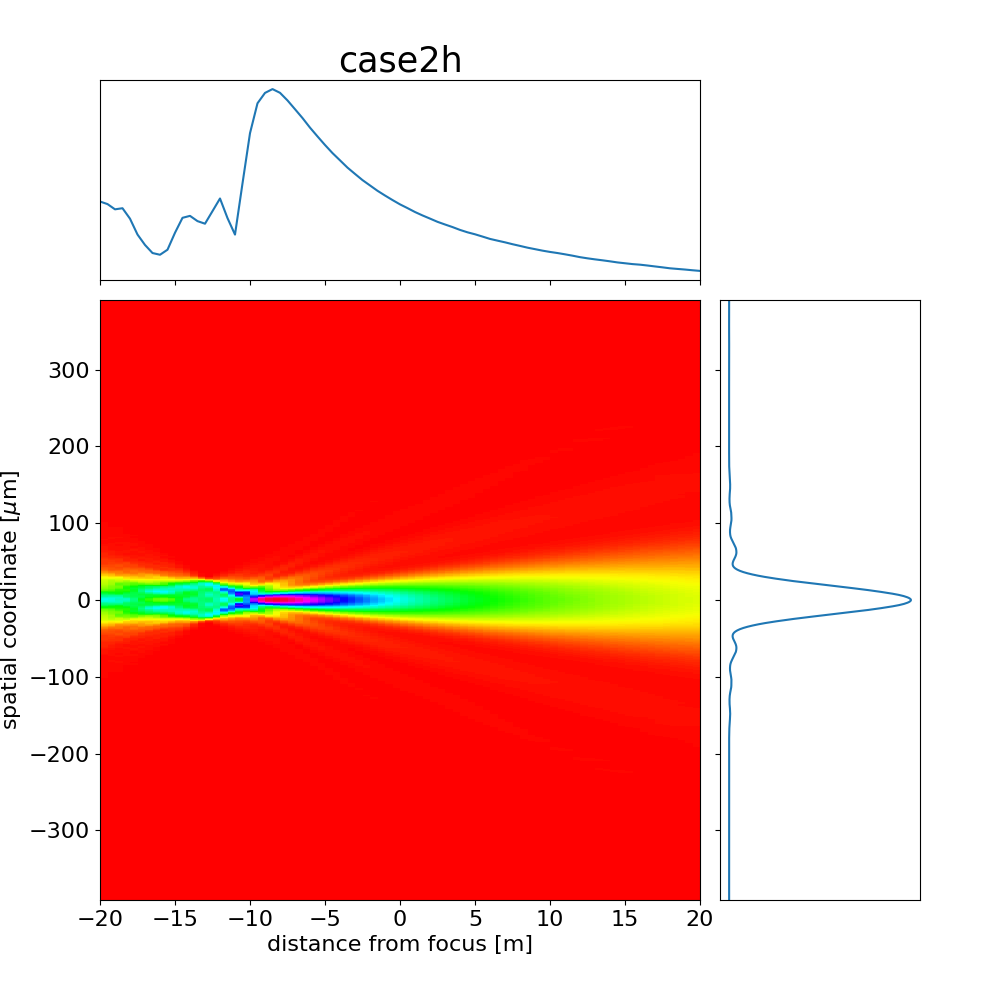
\includegraphics[width=0.49\textwidth]{figures/case2h_caustic.png}
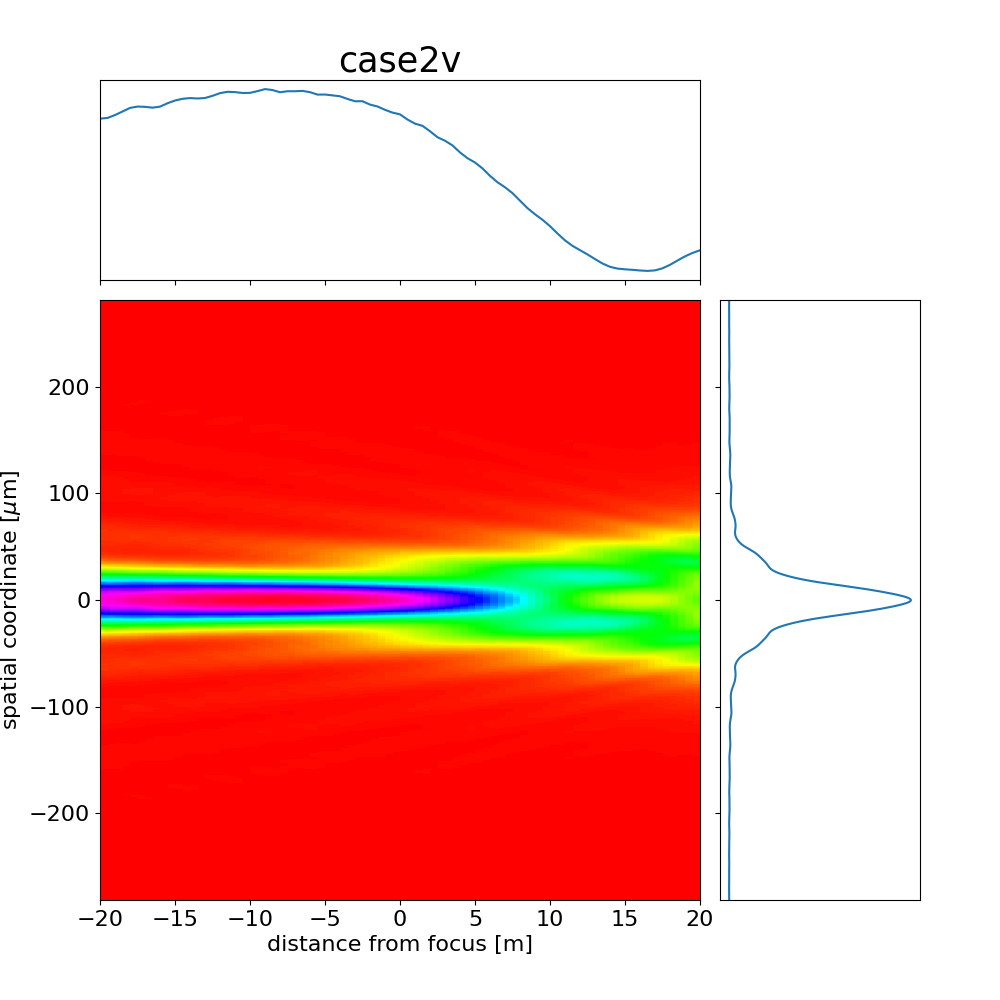
\includegraphics[width=0.49\textwidth]{figures/case2v_caustic.png}

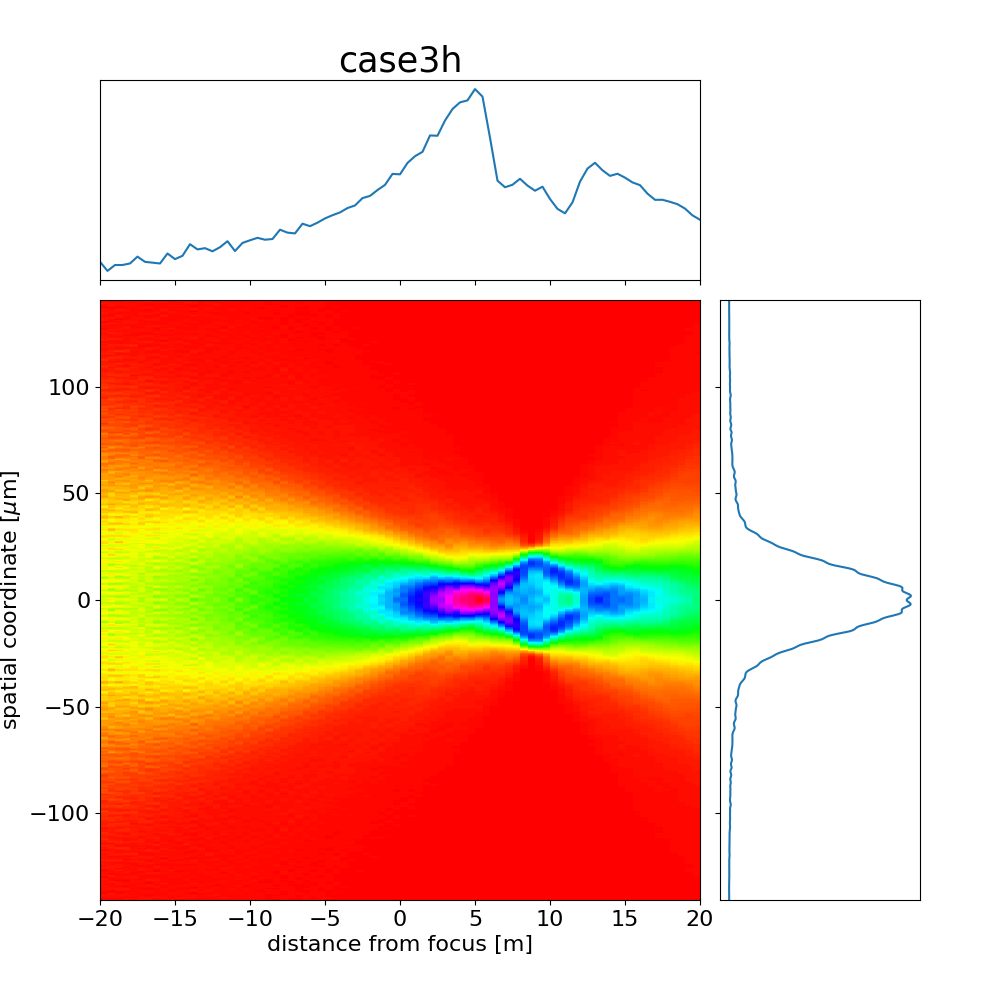
\includegraphics[width=0.49\textwidth]{figures/case3h_caustic.png}
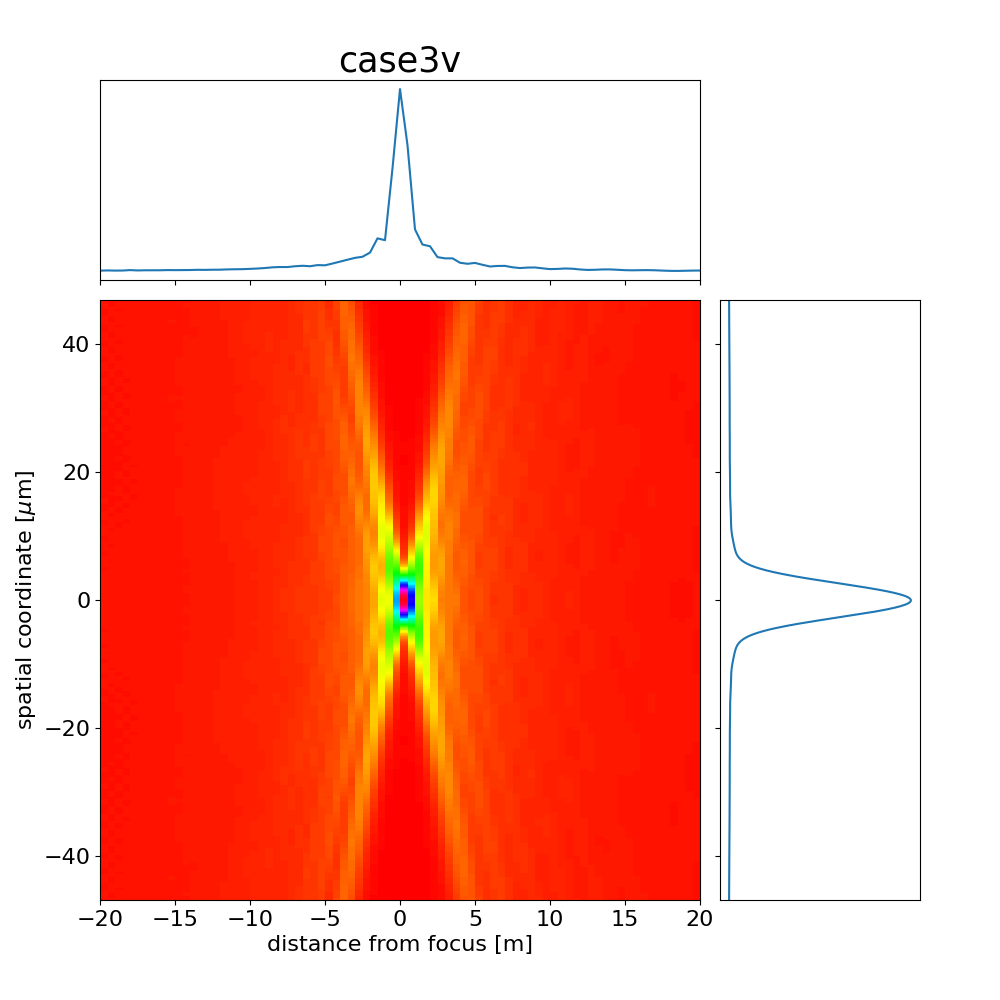
\includegraphics[width=0.49\textwidth]{figures/case3v_caustic.png}

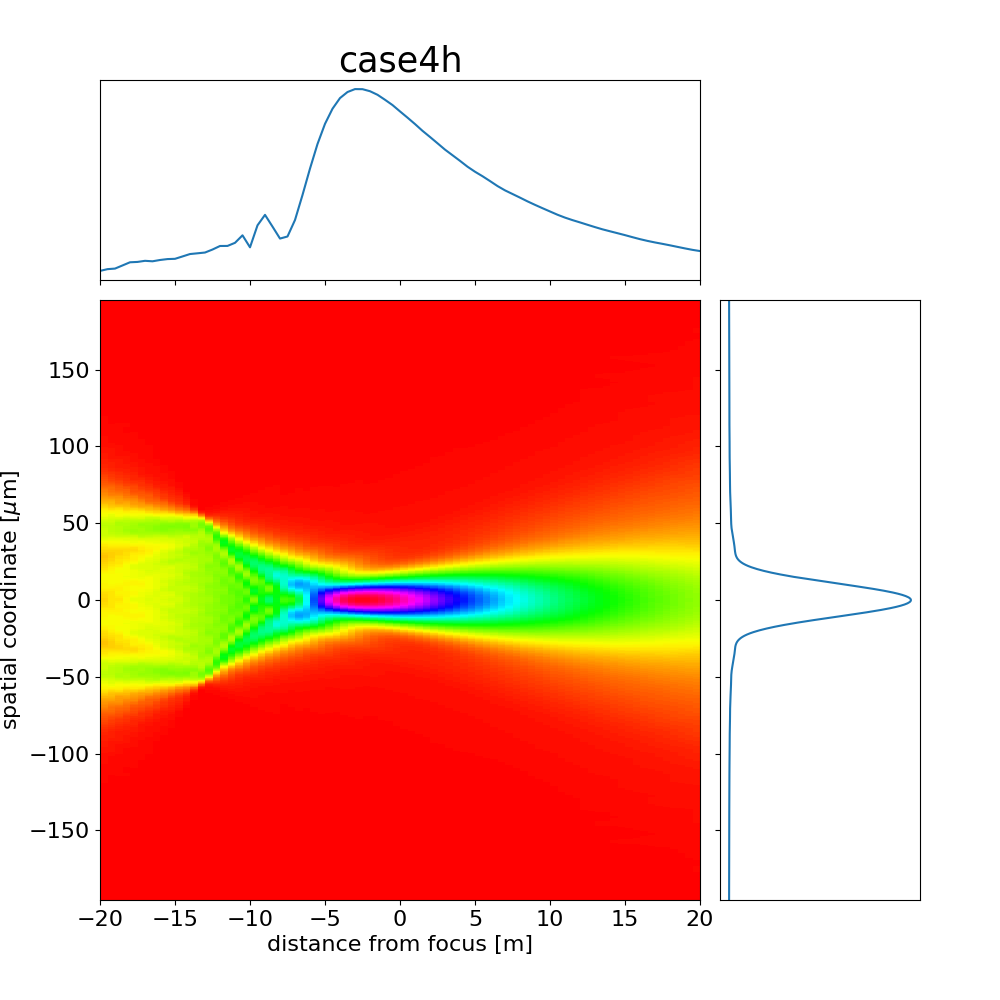
\includegraphics[width=0.49\textwidth]{figures/case4h_caustic.png}
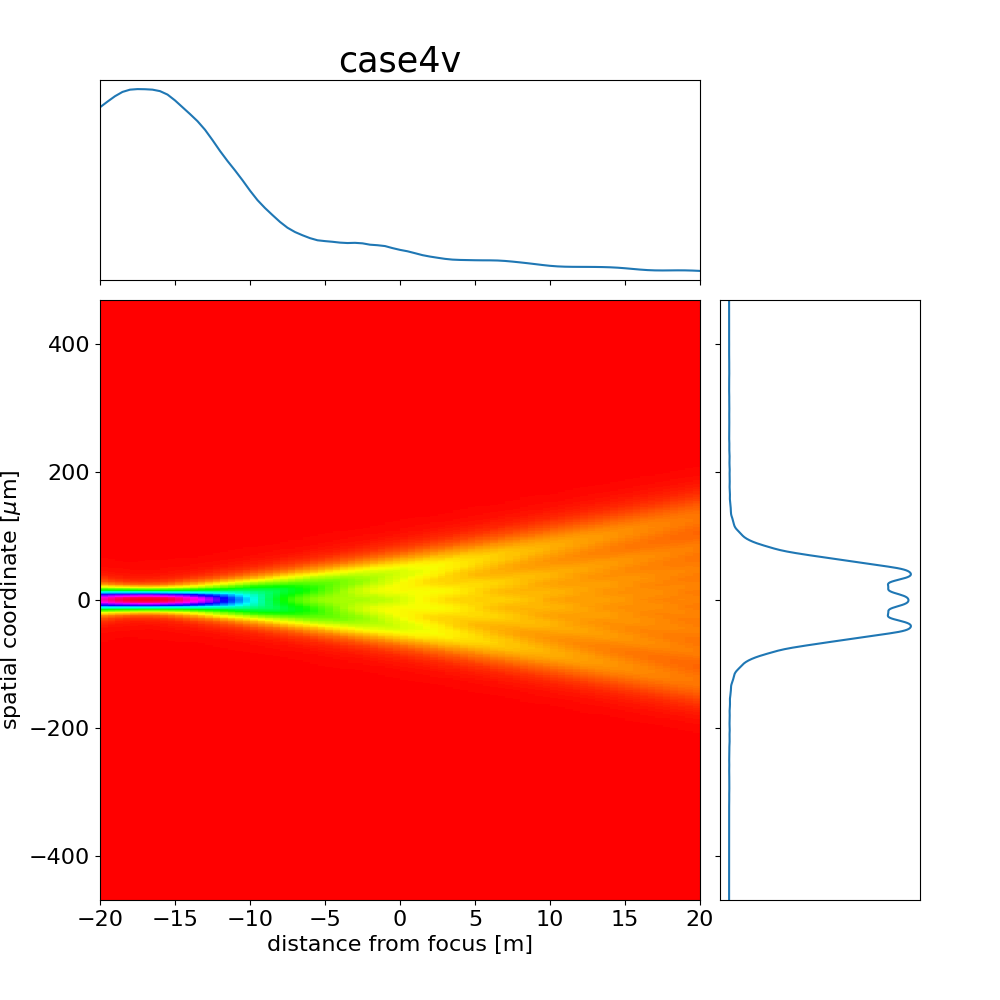
\includegraphics[width=0.49\textwidth]{figures/case4v_caustic.png}

\caption{Evolution of the beam size in the around the sample position for the cases listed in Table~\ref{table:2Dusercases}. The top and side graphs correspond to the profiles passing by (0,0).
}
\end{figure}

%%%%%%%%%%%%%%%%%%%%%%%%%%%%%%%%%%%%%%%%%%%


\begin{figure}\label{fig:causticcorrection}
\centering

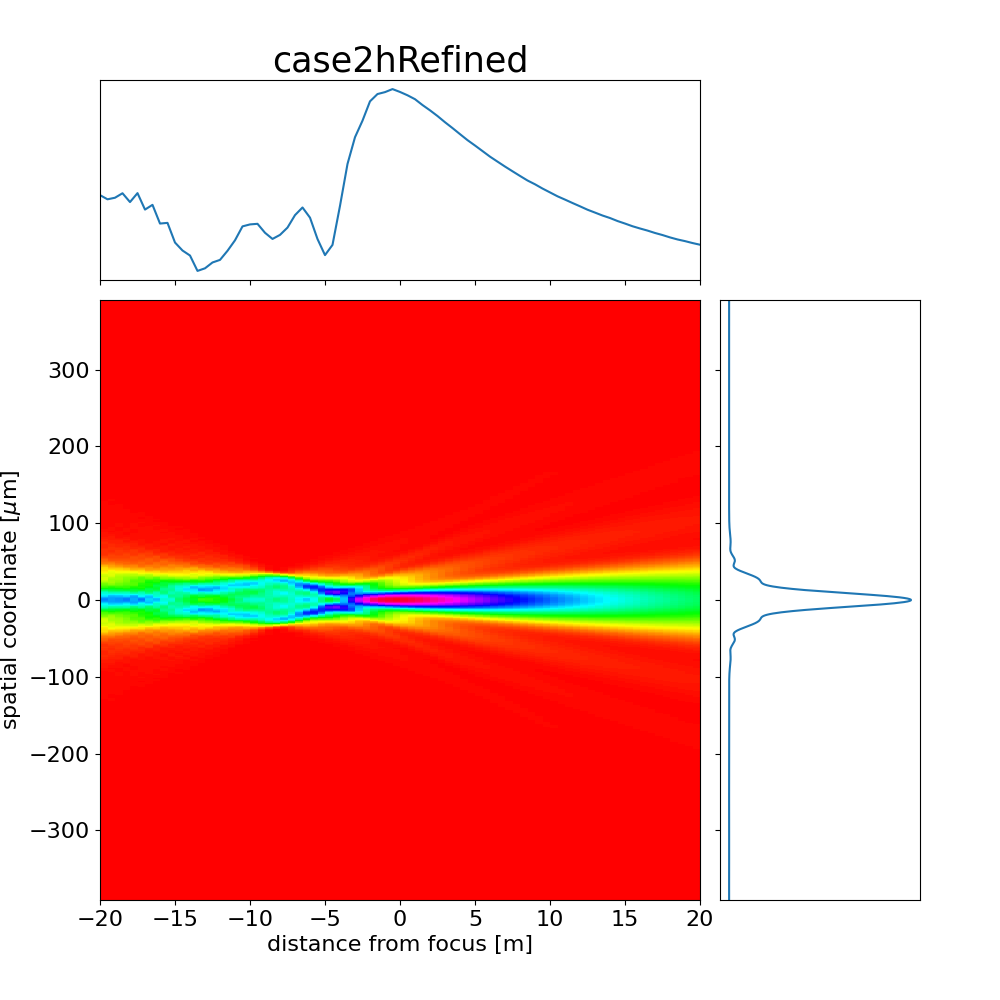
\includegraphics[width=0.49\textwidth]{figures/case2hRefined_caustic.png}
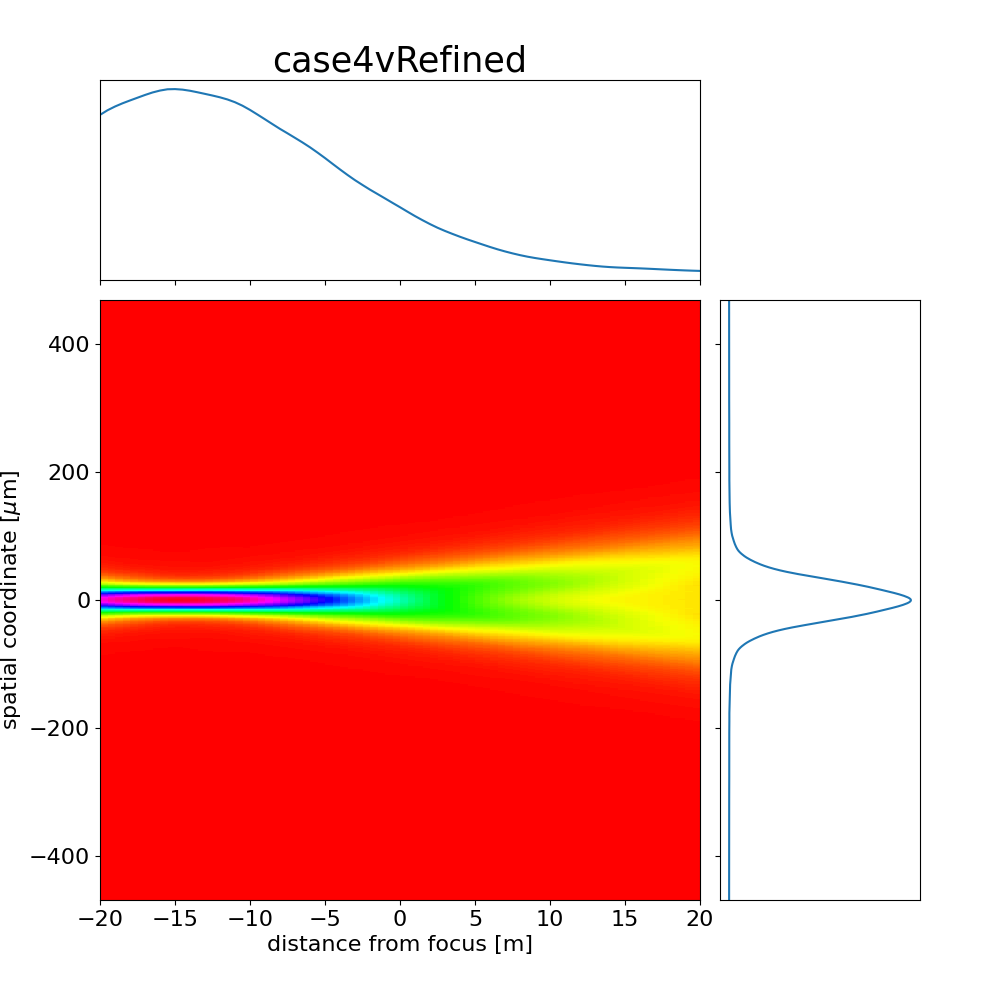
\includegraphics[width=0.49\textwidth]{figures/case4vRefined_caustic.png}
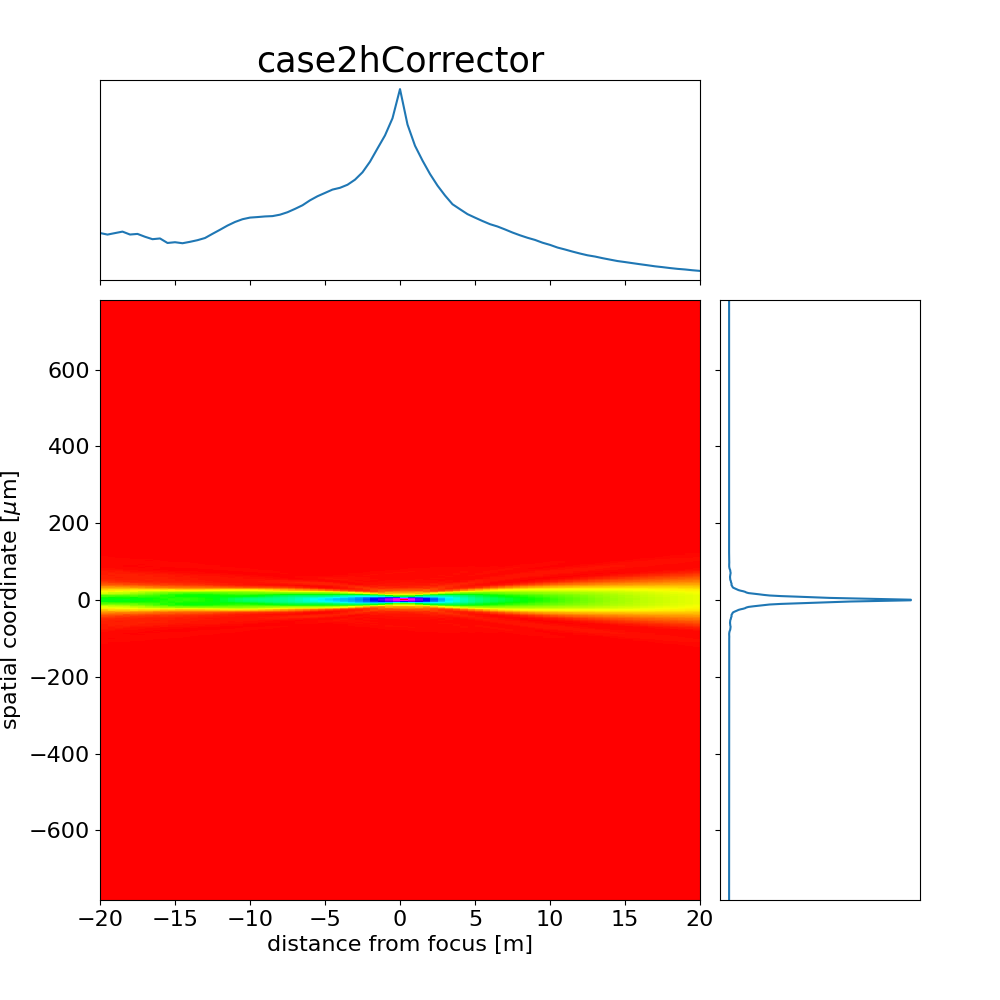
\includegraphics[width=0.49\textwidth]{figures/case2hCorrector_caustic.png}
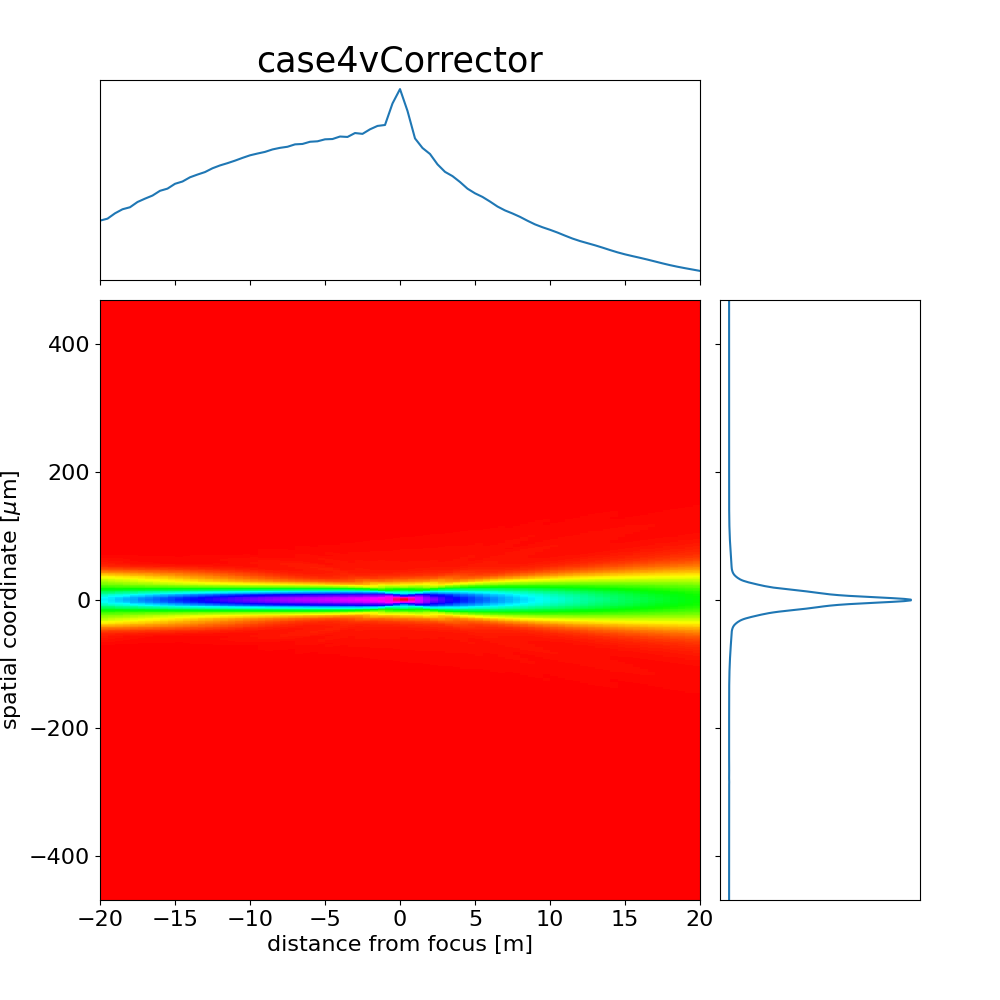
\includegraphics[width=0.49\textwidth]{figures/case4vCorrector_caustic.png}

\caption{Evolution of the beam size in the around the sample position for the ``pathological" case 2h and 4v shown in Fig.~\ref{fig:caustic}. Top row: using corrected lens-2 with $R_2$=\SI{410}{\micro\meter} ($f_2=$\SI{29.4}{\meter}) for case 2h and $R_2=f_2=\infty$ for case 4v. Bottom: using a free-form refractive corrector instead of lens-2.
}
\end{figure}



\subsection{Errors in optical surfaces}

The performance of X-ray optics in the new generation synchrotron beamlines is limited by the quality of the optical surfaces \cite{lengeler1999,Yabashi}. Slope and height errors are often associated with surface finishing (higher spatial frequency), while figure errors are often associated with lower frequency deviations from ideal profile (e.g. bending, gravity sag, thermal deformations) \cite{srio1992, signorato1997}. Figure errors in x-ray lenses can be measured by different techniques (eg. grating interferometry, x-ray speckle tracking or ptychography) and readily included in the simulations \cite{celestre2020}. Some profiles measured at ESRF using x-ray speckle tracking \cite{berujon2020} with height error RMS of the order of \SI{1}{\micro\meter} are used to verify that the focal spot produced by lenses with realistic errors is not degraded with respect to the ideal lens surface. 


% Usually the optics of new generation synchrotron beamlines is limited by the quality of the optical surface. Typically are due to surface finish (slope errors and height errors) and shape errors, often due to heat load. 
% \todo{Rafael, would you please work next paragraph. I checked that your error file (profile 1 in DABAM2D) does not produce relevant changes, thus the odea is to "mention" the errors without presenting a full study.} Surface errors in lens surfaces can be experimentally measured by different techniques (e.g. speckle tracking, ptychography) and included in the simulations. Some profiles measured at ESRF \cite{???} with height error RMS of the order of \SI{1}{\micro\meter}  are used to verify that the focal spot produced by lenses with realistic errors is not degraded with respect to the ideal lens surface. 

\todo{Juan, please read!} The effect of finish surface errors in the white double-mirror system is also analyzed using a measured mirror meridional profile of \SI{2.5}{\nano\meter} height error RMS and \SI{140}{\nano\radian} RMS slope error. 

\todo{Philipp, please read!} The heat load affect several elements of the beamline. For the beamline under consideration, the affected elements (white beam mirrors, and double-crystal monochromators) are not presented in our simulations. Finite element analysis of mirrors and crystals done for other EBS beamlines \cite{Brumund} show that the deformation height profile can be decomposed it two parts: an average bending that is possible to correct by a small readjustment of the focal length of the optical elements downstream the heated element, and a ``residual error" which remain after removing the averaged bending radius, and could only be corrected using adaptive optics. Wofry1D simulations using FEA-generated deformations at the first crystal of a monochromator placed just after the coherent slit showed no significant degradation of the focal spot, both in size and shape. This is mainly due to the low power transmitted by the coherent slit.We checked that the focused beam is almost unchanged when using a profile from FEA analysis with curvature of about \SI{1}{\kilo\meter} and residual slope errors of \SI{30}{\nano\radian}. 



% The deformation profile calculated by FEA \todo{I USED FILE: SRC\_Si\_3.0mrad\_08000eV\_mo\_Si111\_Size1\_nodalOut.out} is is loaded in a ``mirror-like" element in Wofry, as described \cite{srioLBL}. For case 1, a small degradation in the horizontal direction is found (passing from \SI{8.09}{\micro\meter} to \SI{10.21}{\micro\meter} for the first coherent mode). It is accompanied by a loss of symmetry. A large deformation in the vertical spot is observed, but a spot close to the ideal is found when a best circle is subtracted from the profile. It is then possible to correct this added curvature. Indeed, by adjusting $f_2$ \todo{I will calculate this} it is possible to compensate the effects introduced by the crystal bending due to heat load.

\subsection{Selection of the transfocator configuration.} 
The results presented in this paper idealizes the transfocator with two orthogonal single lenses, each one focusing one direction (horizontal of vertical), with parabolic profiles and apex radii adjusted for the wanted focal length (via the usual $f=R/(2 N \delta$). The real transfocator will use a combination of one or several lenses to give a similar radius of curvature  ($R^{-1} = R_1^{-1} + R_2^{-1} + ...$). Two independent transfocators can be used for focusing independently the horizontal and vertical planes. Also, combination of 2D lenses matching the higher radius could be combined with 1D lenses to correct the radius of the direction that requires a shorter focal distance. The combinations of the lenses in the transfocator will not match perfectly the exact focal distances, thus producing a focal position close to the exact focal position at sample location. Depending on the used lenses, a different absorption is due to the accumulated thickness of the individual lenses. For example, the lens radii for case 4 can be obtained in using 2D lenses adjusted to focus in vertical (three lenses with $R_1=$~\SI{5}{\milli\meter}, $R_2=$~\SI{2}{\milli\meter} and $R_3=$~\SI{1}{\milli\meter} to get $R=$~\SI{0.588}{\milli\meter}) then adding two more 1D lenses to adjust the horizontal ($R_1=$~\SI{5}{\milli\meter} and $R_1=$~\SI{1}{\milli\meter} to get $R=$~\SI{0.345}{\milli\meter}, values very close to the exact values from Table~\ref{table:2Dusercases}. We simulated this configuration and got similar profiles than the case studied previously, with small differences in FWHM (10\% or less) and obviously more absorption. The empty space in between the lenses is neglected, which is a good approximation unless effects of ``adiabatic" focusing are expected, which may be the case for sub-micron focii.    

\subsection{Off-resonance.} The simulations considered here where done for monochromatic radiation supposing the undulator tuned at the exact resonance (\SI{7}{keV}). This photon energy may not exactly correspond to the maximum of the emitted flux. Somme effects of out-resonance may appear when i) a ``pink" or not strictly monochromatic beam is used (in beamlines without monochromator or also using a high-band monochomator, as for example using multilayer), or ii) the undulator gap tuned by selecting the maximum of the intensity in a given aperture, thus corresponding to an energy value a bit lower (red-shifted) than exact resonance. The separation from the position of the maximum of intensity to the resonant energy increases when increasing the observation slit. In our case, this beamline will use a slit small enough to gain coherence, which implies that the maximum of the intensity is well approximated by the resonance energy, and it will use a crystal monochromator thus the beam can be considered as monochromatic, thus off-resonance effects are not appreciated. This has been checked numerically by averaging the intensity distribution at the sample position when scanning the photon energy around the resonance value ($7\pm0.1$~keV).   \todo{suppress this paragraph?}


\subsection{The measurement of coherence.} We measured the beam coherence using the coherent fraction $CF$, an idea introduced by \citeasnoun{glass2017}. This parameter has a strict definition in the context of the CMD: $CF$ is the occupation of the first coherent mode ($\eta_0$ in Eq.~\ref{eq:occupation}). We verified that this strict definition give values close to the approximated CF  calculated as the phase space dimension ratio between the coherent undulator emission (zero emittance) over the convolution of the electron beam phase space and the undulator emission. The CMD gives also the possibility of propagating the modes and also recalculate the $CF$ after the slits and optical elements. The coherence slit selects the wanted coherence (90\% for cases 1 and 2; or 70\% for cases 3 and 4 in our study) but the absorption of the lenses can also increase a bit more the coherence at the sample: $CF_h=$~94, 94, 77, 77 $CF_v=$~97, 90, 77, 71 for cases 1, 2, 3 and 4, respectively. 

Other common parameters to define the coherence are the degree of coherence and coherence length. The degree of (transversal) coherence is not a scalar but a function (see equation~\ref{eq:DTC}. The coherence length has not a strict definition and it is usually given as the ``width" of some cut of the coherence degree. We found more intuitive and practical to use the $CF$ as a measure of the coherence. However, a good idea of the coherence length at a given position along the beamline is also given by the FWHM of the first coherence mode (given in brackets in Table~\ref{table:comparison} for the four cases studied).    


% finding focus https://www.optikos.com/finding-focus/
\subsection{Practical considerations} Simulations like those presented here could be very beneficial for beamline operation, for its optimization and quick setting.  Complicated  relationships exist between the beam parameters requested by users (beam size and coherent fraction) and the beamline configuration (undulator, slit and transfocator setting). Quick simulations as done by Wofry1D could be a helpful instrument for the beamline staff to get the desired configurations. The plots shown here (e.g., $CF$ vs slit size in Fig.~\ref{fig:cf_vs_aperture}, trajectories in Fig.~\ref{fig:f1f2map}, or final size in Fig.~\ref{fig:focalSizes} could be simulated on-line and compared with results presented as look-up tables with similar aspect. We are also considering the design of a digital twin that mimics the real transfocator systems to assist beamline setting. For that, the fast simulation using the CMD method developed in Wofry1D will be an integrated component.  

Some practical consequences can be directly deduced from the results shown here. For example, looking at Fig.~\ref{fig:focalSizes} one can observe that the same focal size can be obtained with different configurations. To get a similar size, it is better to prefer a large $f_1$ to avoid over-illuminating the lens-2 and increase transmission of lens-1. The transfocator design is simplified if we restrict the horizontal focal distance t to be smaller than the vertical $f_h>f_v$. Here, $f_v$ can be obtained with lenses focusing in 2D and $f_h$ by adding 1D lenses focusing in the horizontal plane. 

% https://www.optikos.com/finding-focus/
In this work we configured the transfocator to have the resulting focal position on the sample plane, an "in-focus" setup. It could also be possible to work off-focus to vary the beam size at the sample plane. The in-focus setup will generally produce the sharpest image of very small details in the image. Moreover, it will reduce the artifacts produced by the surface finish errors. Also, a larger depth of focus is obtained at this position. To check that, we have propagated the beam at distances close to the focus to see the effect (see Fig. XX). We observe...


\todo{because of the system complexity it would be good to have an experimental method to guarantee that the focus sit on the image plane (so we are not out of focus)}

% \todo{MOVE TO DISCUSSION? This degradation of the focal dimension when focal position cannot be predicted by the geometrical optics adds difficulty to the design of optical systems: the slit must be closed enough to guarantee a good coherence, but opened enough to maintain the focal position not far from that of the geometrical optics.}


\section{Summary and conclusions}
\label{sec:summary}

We have studied in detail the focusing of a partial coherent beam (as produced by the low emittance storage ring EBS-ESRF) by a system of one and two transfocators (or lenses). In agreement with existing works, we observe a displacement of a focal position originated by the reduction of NA. The reduction of NA is the result of closing a slit to gain coherence, a usual procedure in beamlines for X-ray coherence applications. We observed that good focusing (small focus) is obtained when its position coincide with the positions predicted by the geometrical optics (considering the source either at the ID position or at the slit position) but not in intermediate positions (Fig.~\ref{fig:oneTFundPartialCoherence}).

We calculated numerically the map or trajectory of focal distances $(f_1,f_2)$ needed to maintain the focus at the image plane. The beam size values obtained for different cases are very different than those predicted by geometrical optics.  

Numerical calculations for this work have been done using a newly developed method of coherent mode decomposition in 1D. This method is very fast, and many simulations can be run in a laptop, therefore it is ideal for parametric calculations as presented here. This method is available in the Wofry add-on of the OASYS suite \cite{codeOASYS}. Four cases are calculated and compared using the other methods available in OASYS, like the full 2D coherent mode decomposition using COMSYL \cite{codeCOMSYL}, the OASYS interface for the SRW \cite{codeSRW} code, and hybrid ray tracing \cite{codeHYBRID}. OASYS workspaces for the simulations performed in this paper are available at \cite{repository}.

%%%%%%%%%%%%%%%%%%%%%%%%%%%%%%%%%%%%%%%%%%%%%%%%
%%%%%%%%%%%%%%%%%%%%%%%%%%%%%%%%%%%%%%%%%%%%%%%%
%%%%%%%%%%%%%%%%%%%%%%%%%%%%%%%%%%%%%%%%%%%%%%%%
\appendix

%%%%%%%%%%%%%%%%%%%%%%%%%%%%%%%%%%%%%%%%%%%%%%%%


%%%%%%%%%%%%%%%%%%%%%%%%%%%%%%%%%%%%%%%%%%%%%%%%
% \section{One lens: comparison of methods}
% \label{appendix:comparison}


% % \begin{figure}
% %     \centering
% %     \includegraphics[width=0.95\textwidth]{figures/oneTFund_400um.eps}
% %     % \includegraphics[width=0.95\textwidth]{figures/oneTFund_300um.png}  
% %     \includegraphics[width=0.95\textwidth]{figures/oneTFund_200um.eps}
% %     % \includegraphics[width=0.95\textwidth]{figures/oneTFund_100um.png}

% %     \caption{Evolution of the size of a coherent undulator beam cropped by a slit and focused by a lens of different radii values $R$: a) \SI{400}{\micro\meter} and b) \SI{200}{\micro\meter}.
    
% %     }
% %     \label{fig:oneTFundAppendixR}
% % \end{figure}


% \begin{figure}
%     \centering
    
%     a) Und + RectSlit + RealLens \\
%     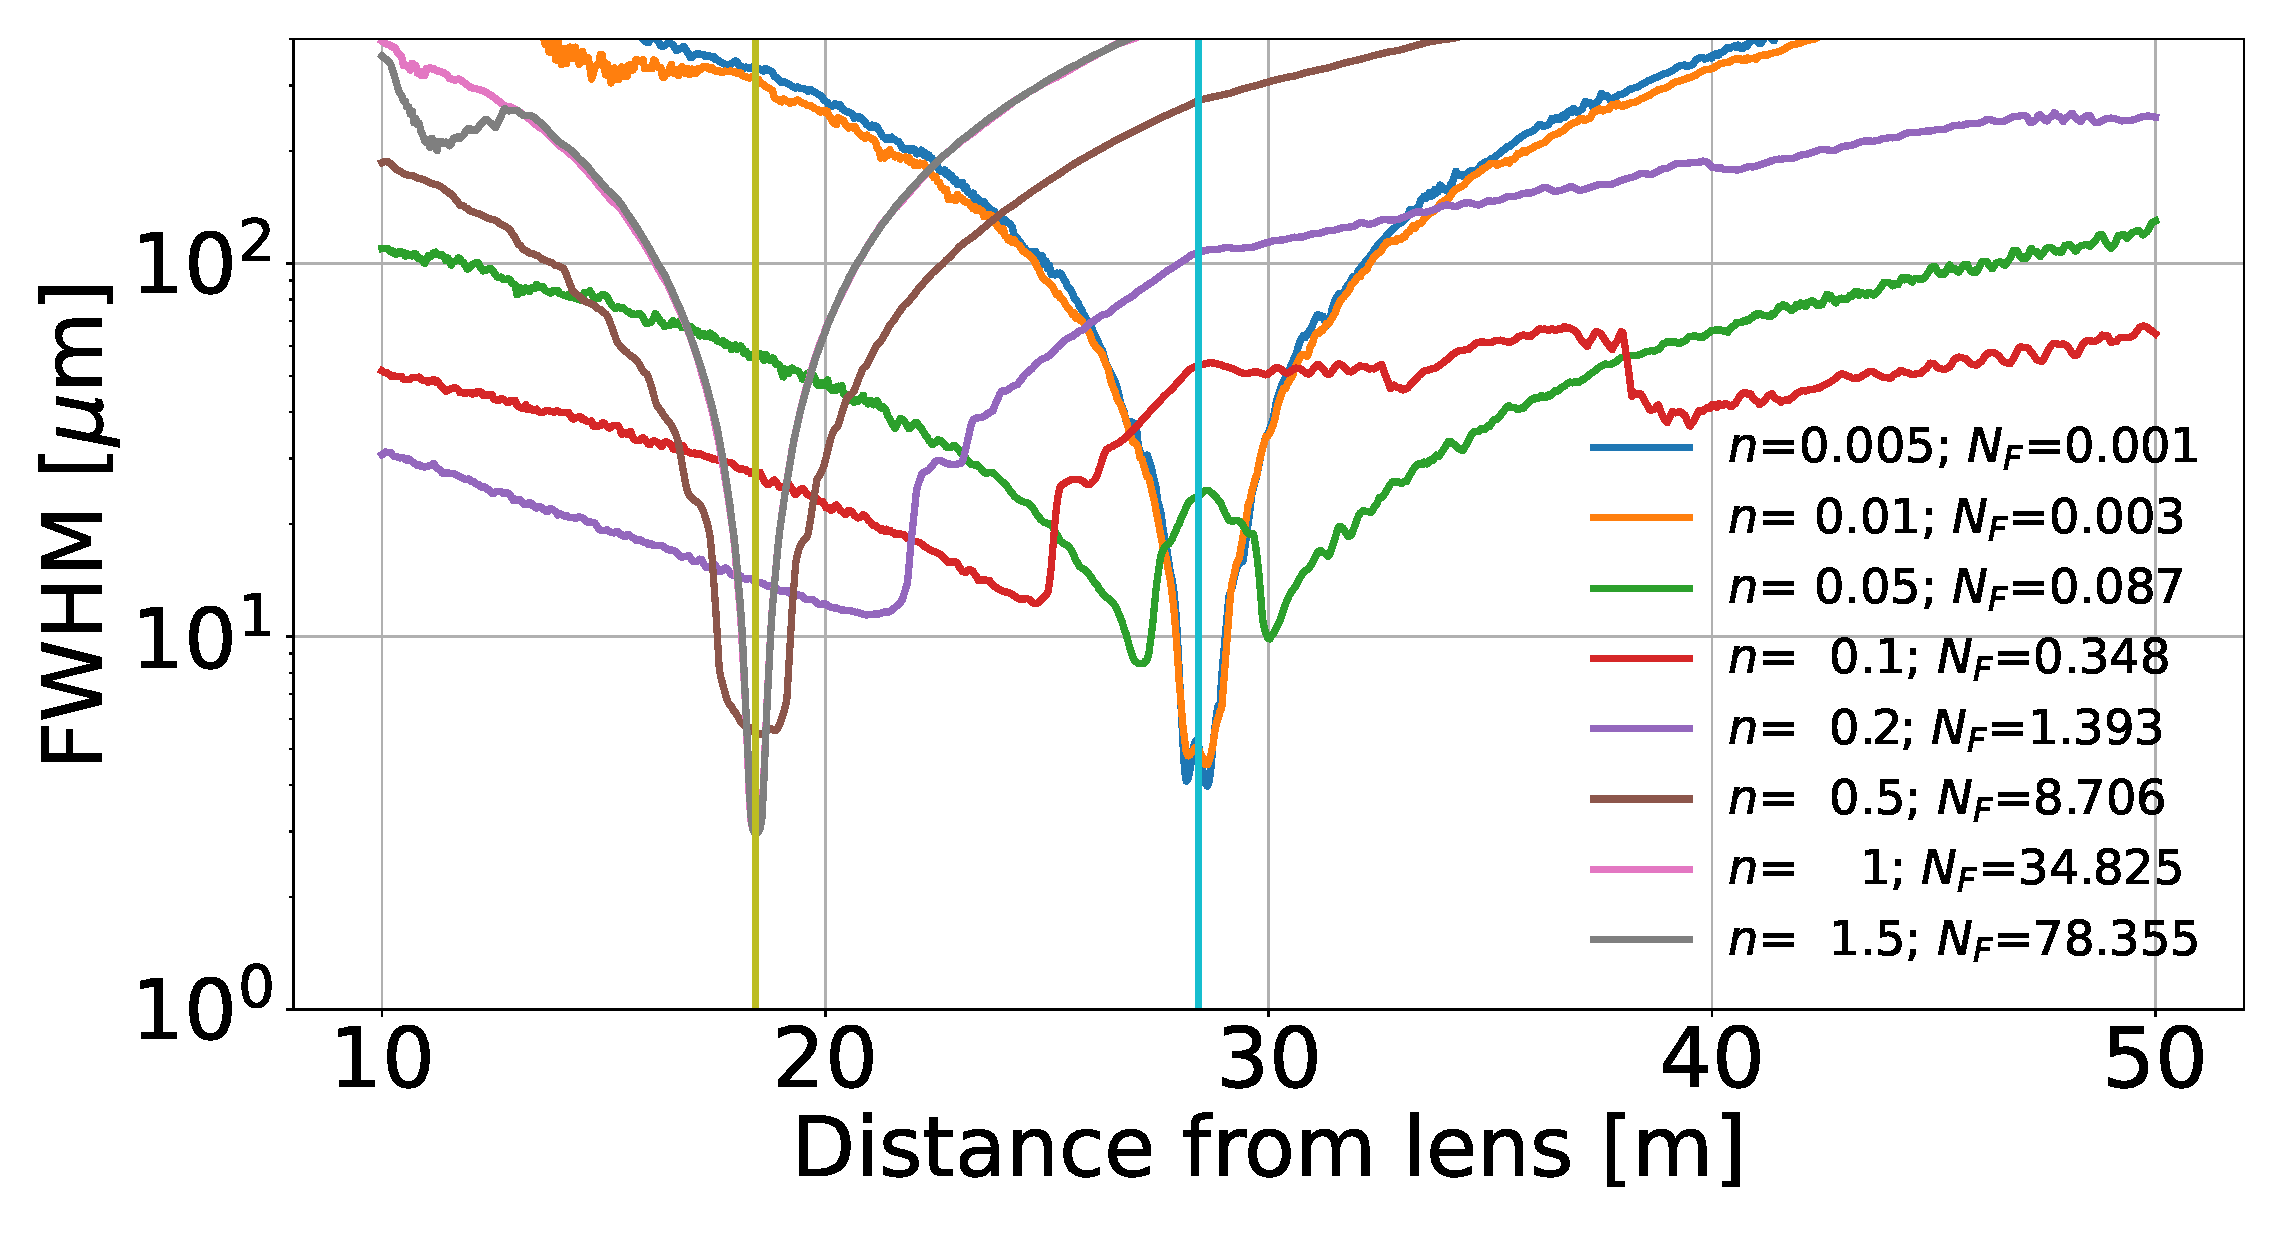
\includegraphics[width=0.95\textwidth]{figures/oneTF_UndSource_RectSlit_R200um.eps}
    
%     b) Gauss + RectSlit + RealLens \\
%     \includegraphics[width=0.95\textwidth]{figures/oneTF_GaussianSource_RectSlit_R200um.eps}
    
%     c) Gauss + GaussSlit + RealLens \\
%     \includegraphics[width=0.95\textwidth]{figures/oneTF_GaussianSource_GaussianSlit_200um.eps}

%     d) Gauss + GaussSlit + IdealLens \\
%     \includegraphics[width=0.95\textwidth]{figures/oneTF_GaussianSource_GaussianSlit_IdealLens.eps}
    
%     e) Hybrid (Und + RectSlit + RealLens) \\
%     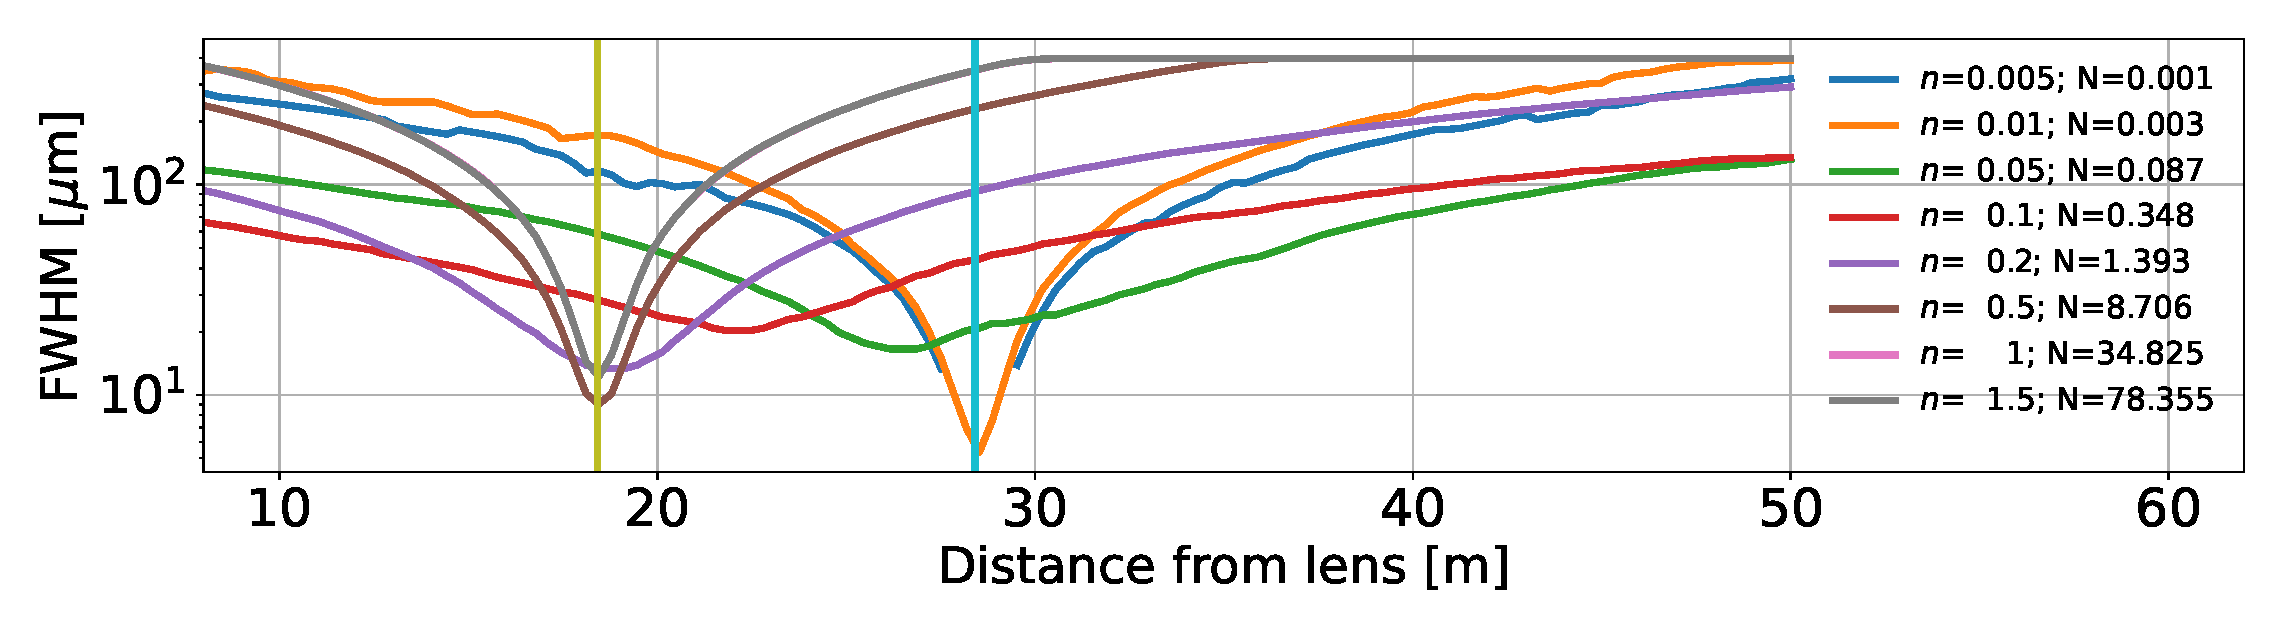
\includegraphics[width=0.95\textwidth]{figures/oneTF_ShadowHybrid_R200um.eps}
    
%     \caption{Evolution of the size of a coherent undulator beam cropped by a slit and focused by a lens of $R$=~\SI{0.2}{\milli\meter} using different methods: 
    
%     a) Undulator source + Rectangular Slit + Real Lenses
    
%     b) Gaussian source + Rectangular Slit + Real Lenses
    
%     c) Gaussian source + Gaussian Slit + Real Lenses
        
%     d) Gaussian source + Gaussian Slit + Ideal lens (Full Gaussian)
        
%     e) Ray tracing, hybrid, with undulator source + Rectangular Slit + Real Lenses.
%     }
%     \label{fig:oneTF_comparison}
% \end{figure}


% \begin{figure}

%     \includegraphics[width=0.95\textwidth]{figures/waist_size_comparison.eps}
    
%     \caption{Waist size vs slit aperture for the different methods studied. 
    
%     }
% \end{figure}

% \section{SRW-ME convergence}
\newpage
\section{Some considerations on partially-coherent calculations using SRW's macro-electrons \& simulation convergence}
\label{appendix:srw}
In the frequency domain, the synchrotron radiation (SR) intensity from $N_\text{e}$ electrons is given by: 
\begin{equation}
\begin{split}
|E&_{\omega\text{~bunch}}(\textbf{r})|^2 \approx \\
 &N_\text{e} \int\big| E_\omega(\textbf{r};\textbf{s}_\text{e}, \textbf{s}'_\text{e}, \gamma_\text{e})\big|^2\cdot f(\textbf{s}_\text{e}, \textbf{s}'_\text{e}, \gamma_\text{e})~ \text{d}\textbf{s}_\text{e} \text{d}\textbf{s}'_\text{e} \text{d}\gamma_\text{e}~+\\
&+~ N_\text{e}(N_\text{e}-1)\bigg| \int E_\omega(\textbf{r};\textbf{s}_\text{e}, \textbf{s}'_\text{e}, \gamma_\text{e})\cdot f(\textbf{s}_\text{e}, \textbf{s}'_\text{e}, \gamma_\text{e})~ \text{d}\textbf{s}_\text{e} \text{d}\textbf{s}'_\text{e} \text{d}\gamma_\text{e} \bigg|^2,
\end{split}
\label{eq:SR}
\end{equation}
where $E_{\omega\text{~bunch}}(\textbf{r})\equiv E_{\text{~bunch}}(x,y;\omega)$ and $E_\omega(\textbf{r})\equiv E(x,y;\omega)$; $\textbf{s}_\text{e}=(x_\text{e},y_\text{e},z_\text{e})$ represents the electron initial positions, $\textbf{s}'_\text{e}=(x'_\text{e},y'_\text{e})$ gives the electron initial directions and $\gamma_\text{e}$ is the electron energy. All sampled from the 6D electron-beam phase-space such that $\int f(\textbf{s}_\text{e}, \textbf{s}'_\text{e}, \gamma_\text{e})~ \text{d}\textbf{s}_\text{e} \text{d}\textbf{s}'_\text{e} \text{d}\gamma_\text{e}=1$ \cite{codeSRW_CSR}. The methods for computing the spontaneous emission by a relativistic electron submitted to an arbitrary magnetic field, that is $E_\omega(\textbf{r};\textbf{s}_\text{e}, \textbf{s}'_\text{e}, \gamma_\text{e})$, are described in \cite{Chubar1995,codeSRW}.
The first term in the sum from Eq.~\ref{eq:SR} describes temporally incoherent SR, while the second term, temporally coherent SR: $\text{I}_\text{~bunch} = \text{I}_\text{~iSR}+\text{I}_\text{~cSR}$. For emitted wavelengths shorter than the electron bunch length, the power associated with the term $\text{I}_\text{~cSR}$ vanishes quickly \cite{Wiedemann2015}. At typical X-ray energy ranges in the ESRF-EBS, i.e. from a few hundred electron-volts to a few hundred keV, and typical bunch lengths (over 30~ps), cSR can be completely neglected even when considering standard monochromatisation schemes in beamlines. A further simplification to Eq.~\ref{eq:SR} is done when considering that the intensity of the single-electron emission is not dependent on the initial electron position $z_\text{e}$. The integration of Eq.~\ref{eq:SR} can then be done in 5 dimensions.

The SRW-ME algorithm used to account for partial (transverse) coherence implements Eq.~\ref{eq:SR} by individually calculating the SR emission of several electrons subjected to the initial conditions sampled from $f(\textbf{s}_\text{e}, \textbf{s}'_\text{e}, \gamma_\text{e})$ passing through an arbitrary magnetic field describing the X-ray source. Each resulting electric field is then propagated through the beamline until the observation point, where the contributions from different electrons are added in intensity \cite{codeSRW_ME}. It is impractical (and unnecessary) to account for the emission of every single electron in a beam that very often has a current of few hundreds mA. Electrons are then divided in so-called macro-electrons (\textit{me's}), which is an abstraction that allows to group the emission of several individual electrons into one particle behaving (in electro-dynamics theory terms) as a single electron emission, but with resulting intensity given by the total intensity $\text{I}_\text{~bunch}$ divided by the number of macro-electrons. An advantage of the SRW-ME approach is that the electric fields of the \textit{me's} propagate independently from each other, which allows a convenient parallelisation of the wavefront propagations among many processors.

The convergence of this method is based on the \textit{finesse} with which the distribution $f(\textbf{s}_\text{e}, \textbf{s}'_\text{e}, \gamma_\text{e})$ is sampled. While an exquisitely large number of \textit{me's} will lead to a more accurate simulation, the resulting calculation would be very long and impossible to be performed on personal computers within reasonable time even if performed in parallel. The number of \textit{me's} depends on overall beamline degree of coherence at the observation plane, which is impacted by the source coherent fraction and beamline overall transmission (eg. slits, creation of secondary sources or any other spatial filtering scheme). Special attention to the number of macro-electrons should be given if the simulation accounts for vibrations in the beamline elements or broad-band radiation (eg. pink beam or radiation filtered by multi-layer monochromators).

To illustrate the effect of the number of macro-electrons on the beam profile we choose the previously studied cases 1 and 3 from \S\ref{sec:complete-beamline} - due to their CF, cases 2 and 4 are expected to have the same convergence as 1 and 3, respectively. Both systems 1 \& 3 (and 2 \& 4) have the same X-ray source and are illuminated up until the slits (36~m downstream U18) by the same beam, differing mainly by the coherent fraction selected for the rest of the beamline with case 1 having a higher CF than case 3 - refer to Tables~\ref{table:id18parameters} and \ref{table:2Dusercases} for the complete simulation parameters. The results for a selected number of \textit{me's} are shown in Figs.~\ref{fig:me_c1} and \ref{fig:me_c3}. The 1 \textit{me} simulation represents the filament-beam source, where the electron beam emittance is negligible and the fully spatial coherence is assumed - this is often called a "single electron simulation". On the other extreme, an exaggerated value of 100k $me's$ is chosen as a way of guaranteeing convergence by brutal-force. Two criteria are used to evaluate the convergence of the simulations: the beam shape and peak intensity stabilisation. The profile cuts in  Fig.~\ref{fig:me_c1}(a)-(b) and Fig.~\ref{fig:me_c3}(a)-(b) show that the profile shape starts to converge to that of a 100k $me's$ after $\sim$500 macroelectrons for case 1 and $\sim$1k macroelectrons for case 3. Beyond that, it is necessary to resort to the relative error standard deviation and the peak intensity stabilisation. Fig.~\ref{fig:me_c1}(c)-(d) and Fig.~\ref{fig:me_c3}(c)-(d) show that for both cases, the convergence happens between 2k and 5k $me's$. Further increase in the number of macro electrons does not translate in improvements in the simulations (see simulations for 10k $me's$ onward), but increase greatly the cost of the calculation as shown in Fig.~\ref{fig:me_t}. For the work presented here a good compromise between accuracy and efficiency of the calculations is reached at 5k $me's$. Other factors contributing to the total elapsed simulation time and overall parallel performance of SRW-ME method are presented in \S3.3 from \cite{codeSRW_MEscan}, but these do not impact the SRW-ME convergence.

It is important to note that this large scan procedure is merely illustrative. Usually an experienced optical designer starts with a good guess of the necessary number of $me's$ based on the characteristics of the source (degree of coherence) and optical system (transmission and expected degree of coherence at the observation plane). This choice usually includes considerations of time and resources consumption. If there are signs that the choice may be too low, further attempts with higher $me's$ should be done. If the simulation looks fine from the first guess, reducing the number of $me's$ is also interesting as very often it is necessary to repeat the simulations (eg. testing different configurations, different energies, tolerancing or even different observation planes). At the time of writing, the authors are unaware of any widespread metric within the SRW's community capable of giving the exact number of \textit{me's} necessary for the convergence of the SRW-ME method other than the $me's$ scan. We welcome the discussion on SRW-ME convergence and we encourage the reader to reach out if they employ any interesting and reproducible convergence metric that is less time (and resource) consuming.

% \begin{table}[]
% \label{table:me_t}
% \caption{Time}
% \resizebox{\textwidth}{!}{
% \begin{tabular}{cccccccc}
%  & 500 & 1k & 2k & 5k & 10k & 25k & 100k \\ \hline
% case 1: & 5min & 9min & 15min & 39min & 1h20min & 3h21min & 13h15min \\
% case 3: & 9min & 17min & 30min & 1h15min & 2h35min & 6h30min & 35h39min
% \end{tabular}}
% \end{table}

\begin{figure}
    \centering
    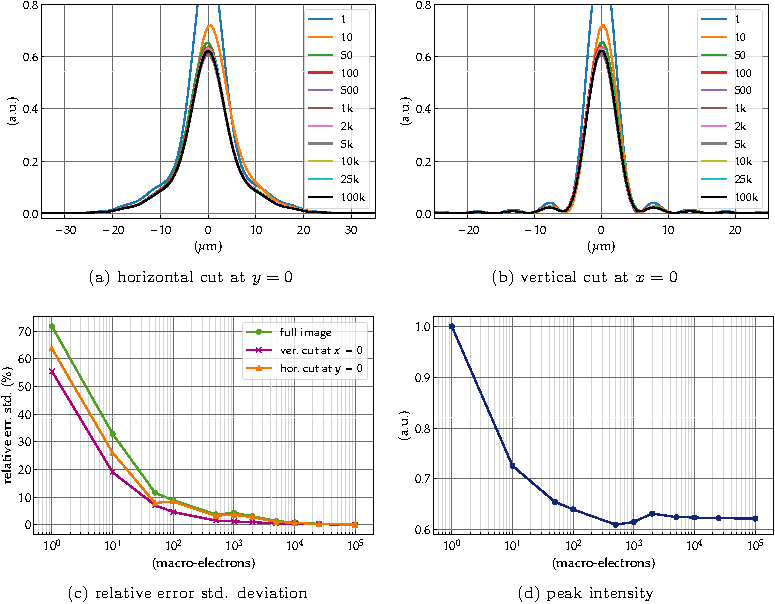
\includegraphics[width=10cm]{figures/c1.pdf}
    \caption{Partially-coherent simulations convergence study: case 1. (a) horizontal and (b) vertical intensity cuts at E=7~keV for $me's$ ranging from 1 to 100k. (c) errors relative to the $me's=$100k plots and (d) peak intensity.}
    \label{fig:me_c1}
\end{figure}

\begin{figure}
    \centering
    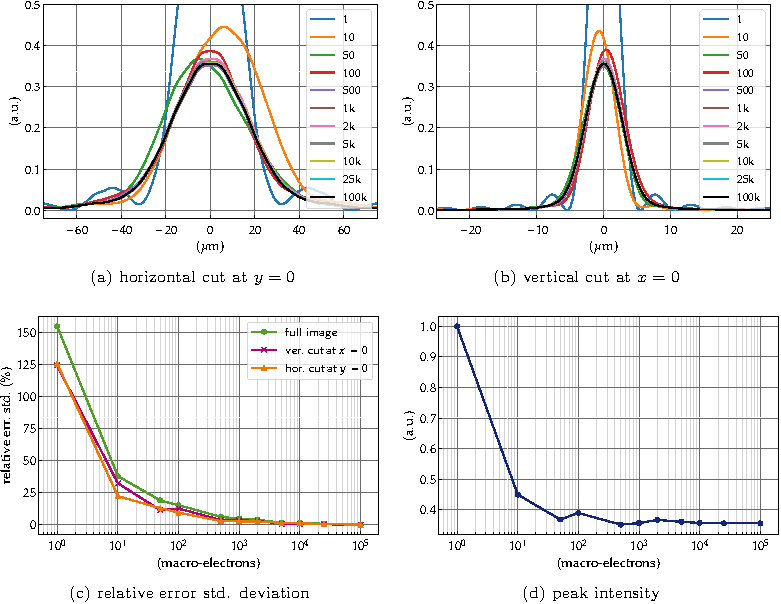
\includegraphics[width=10cm]{figures/c3.pdf}
    \caption{Partially-coherent simulations convergence study: case 3. (a) horizontal and (b) vertical intensity cuts at E=7~keV for $me's$ ranging from 1 to 100k. (c) errors relative to the $me's=$100k plots and (d) peak intensity.}
    \label{fig:me_c3}
\end{figure}

\begin{figure}
    \centering
    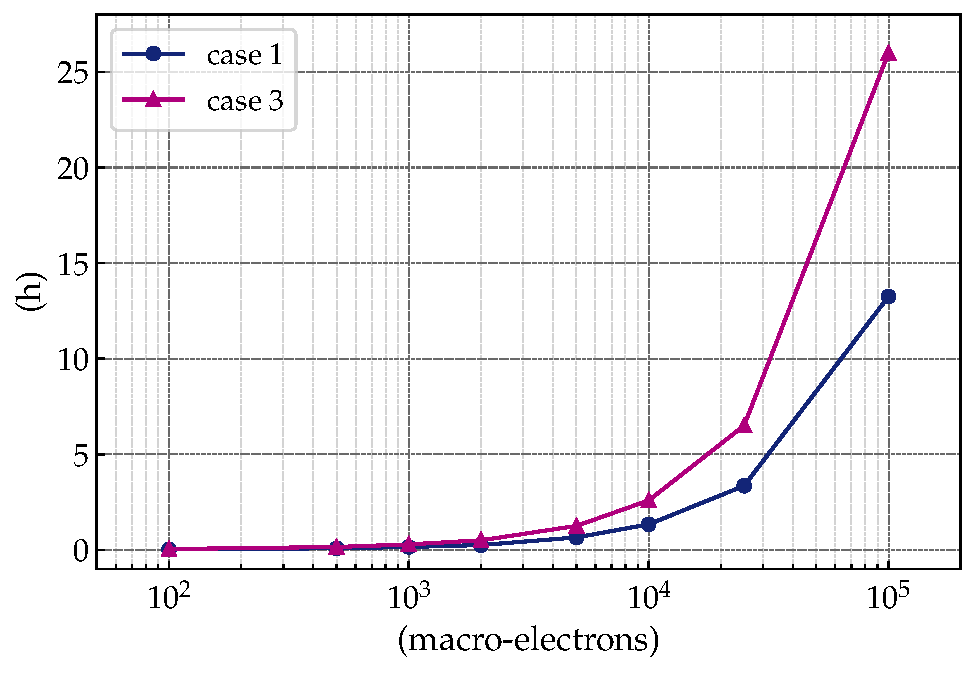
\includegraphics[width=5cm]{figures/srw_time.pdf}
    \caption{Total elapsed time for partially-coherent simulations using a computer cluster with 28 processors for parallel calculations as a function of number of $me's$.}
    \label{fig:me_t}
\end{figure}

\newpage
% %%%%%%%%%%%%%%%%%%%%%%%%%%%%%%%%%%%%%%%%%%%%%%%%
% %%%%%%%%%%%%%%%%%%%%%%%%%%%%%%%%%%%%%%%%%%%%%%%%
% %%%%%%%%%%%%%%%%%%%%%%%%%%%%%%%%%%%%%%%%%%%%%%%%

     %-------------------------------------------------------------------------
     % The back matter of the paper - acknowledgements and references
     %-------------------------------------------------------------------------

     % Acknowledgements come after the appendices

\ack{Acknowledgements}

     % References are at the end of the document, between \begin{references}
     % and \end{references} tags. Each reference is in a \reference entry.

% \begin{references}
% \reference{Author, A. \& Author, B. (1984). \emph{Journal} \textbf{Vol}, 
% first page--last page.}
% \end{references}
% \cite{knuth84}

%% Note added by Overleaf: If using bibtex, remove the "references" environment above, and uncomment the following lines.
\bibliographystyle{iucr}
\referencelist{iucr}

     %-------------------------------------------------------------------------
     % TABLES AND FIGURES SHOULD BE INSERTED AFTER THE MAIN BODY OF THE TEXT
     %-------------------------------------------------------------------------

     % Simple tables should use the tabular environment according to this
     % model

% \begin{table}
% \caption{Caption to table}
% \begin{tabular}{llcr}      % Alignment for each cell: l=left, c=center, r=right
%  HEADING    & FOR        & EACH       & COLUMN     \\
% \hline
%  entry      & entry      & entry      & entry      \\
%  entry      & entry      & entry      & entry      \\
%  entry      & entry      & entry      & entry      \\
% \end{tabular}
% \end{table}

     % Postscript figures can be included with multiple figure blocks

% \begin{figure}
% \caption{Caption describing figure.}
% \includegraphics{fig1}
% \end{figure}


\end{document}                    % DO NOT DELETE THIS LINE
%%%%%%%%%%%%%%%%%%%%%%%%%%%%%%%%%%%%%%%%%%%%%%%%%%%%%%%%%%%%%%%%%%%%%%%%%%%%%%
